% =====================================================================
%  Voice-Control for Drone Swarms via Small Language Models
%  Product Requirements Document -- Execution Specification (v2.0)
%
%  Engine   : pdflatex  (also compiles with lualatex / xelatex)
%  Passes   : 3  (TOC + hyperref + longtable need multiple passes)
%  Build    : python build_pdf.py
%  Check    : python check_tex.py docs/PRD.tex
%  Packages : standard TeX Live / MiKTeX -- no exotic dependencies
% =====================================================================
\documentclass[11pt,a4paper]{article}

% ---------------- encoding & fonts ----------------
\usepackage[T1]{fontenc}
\usepackage[utf8]{inputenc}
\usepackage{lmodern}
\usepackage{microtype}

% ---------------- page layout ----------------
\usepackage[a4paper,margin=2.2cm,headheight=15pt,includeheadfoot]{geometry}
\usepackage{fancyhdr}
\usepackage{titlesec}
\usepackage{enumitem}

% ---------------- maths & symbols ----------------
\usepackage{amsmath}
\usepackage{amssymb}

% ---------------- tables ----------------
\usepackage{booktabs}
\usepackage{longtable}
\usepackage{array}
\usepackage{ragged2e}

% ---------------- graphics ----------------
\usepackage{xcolor}
\usepackage{graphicx}
\usepackage{tikz}
\usetikzlibrary{positioning,arrows.meta,fit,backgrounds}

% ---------------- code listings ----------------
\usepackage{listings}

% ---------------- captions ----------------
\usepackage[font=small,labelfont=bf,skip=4pt]{caption}

% ---------------- hyperlinks (load late) ----------------
\usepackage[hidelinks,breaklinks=true]{hyperref}

% =====================================================================
%  Style definitions
% =====================================================================
\definecolor{accent}{RGB}{0,84,145}
\definecolor{rulegray}{RGB}{185,190,196}
\definecolor{codebg}{RGB}{246,247,249}
\definecolor{panelbg}{RGB}{234,241,247}

\setlength{\tabcolsep}{4pt}
\renewcommand{\arraystretch}{1.18}
\setlength{\LTcapwidth}{\textwidth}

\newcolumntype{P}[1]{>{\RaggedRight\arraybackslash}p{#1\textwidth}}

\newcommand{\code}[1]{{\ttfamily\small #1}}
\newcommand{\yes}{$\checkmark$}
\newcommand{\munit}[1]{\,#1}

\titleformat{\section}{\normalfont\Large\bfseries\color{accent}}{\thesection}{0.75em}{}
\titleformat{\subsection}{\normalfont\large\bfseries}{\thesubsection}{0.65em}{}
\titlespacing*{\section}{0pt}{2.4ex plus 1ex minus .2ex}{1.3ex plus .2ex}
\titlespacing*{\subsection}{0pt}{1.8ex plus .8ex minus .2ex}{0.9ex plus .2ex}

\pagestyle{fancy}
\fancyhf{}
\fancyhead[L]{\small\itshape Voice-Control for Drone Swarms --- Execution PRD}
\fancyhead[R]{\small ESI-SBA \textbar{} IASD 2025/2026}
\fancyfoot[C]{\small\thepage}
\renewcommand{\headrulewidth}{0.4pt}
\renewcommand{\headrule}{\hbox to\headwidth{\color{rulegray}\leaders\hrule height \headrulewidth\hfill}}

\lstdefinestyle{panel}{%
  basicstyle=\ttfamily\footnotesize,
  breaklines=true,
  breakatwhitespace=false,
  columns=fullflexible,
  keepspaces=true,
  showstringspaces=false,
  frame=single,
  framerule=0.4pt,
  rulecolor=\color{rulegray},
  backgroundcolor=\color{codebg},
  framesep=5pt,
  xleftmargin=7pt,
  xrightmargin=7pt,
  aboveskip=9pt,
  belowskip=9pt,
  numbers=none,
}
\lstset{style=panel}

% framed info panel (savebox pattern -- supports multiple paragraphs)
\newsavebox{\panelbox}
\newenvironment{panel}
  {\par\begin{center}\begin{lrbox}{\panelbox}\begin{minipage}{0.94\textwidth}\vspace{3pt}}
  {\vspace{3pt}\end{minipage}\end{lrbox}%
   \fcolorbox{rulegray}{panelbg}{\usebox{\panelbox}}\end{center}\par}

% =====================================================================
\begin{document}

% ---------------------------------------------------------------- title
\begin{titlepage}
\centering
\vspace*{0.4cm}

{\small R\'EPUBLIQUE ALG\'ERIENNE D\'EMOCRATIQUE ET POPULAIRE\par
MINIST\`ERE DE L'ENSEIGNEMENT SUP\'ERIEUR ET DE LA RECHERCHE SCIENTIFIQUE\par}

\vspace{0.8cm}
{\large\bfseries \'ECOLE SUP\'ERIEURE EN INFORMATIQUE --- SIDI BEL ABB\`ES\par}

\vspace{0.3cm}
{\small D\'epartement: Second Cycle \quad\textbullet\quad Sp\'ecialit\'e: IASD\par
Ann\'ee universitaire: 2025/2026 \quad\textbullet\quad Projet de Fin d'\'Etudes\par}

\vspace{1.6cm}
{\color{rulegray}\hrule height 1.2pt}
\vspace{0.9cm}

{\Huge\bfseries\color{accent} Voice-Control for Drone Swarms\par}
\vspace{0.45cm}
{\LARGE via Small Language Models\par}
\vspace{0.55cm}
{\large\itshape Edge-Deployed Structured Command Parsing on a Raspberry Pi 5\par}

\vspace{0.9cm}
{\color{rulegray}\hrule height 1.2pt}
\vspace{1.3cm}

{\large\bfseries Product Requirements Document\par}
\vspace{0.2cm}
{\large Execution Specification --- Version 2.0\par}

\vspace{1.7cm}

\begin{tabular}{@{}P{0.26}P{0.60}@{}}
\toprule
\textbf{Student}            & Tayeb Kahia \\
\textbf{Supervisor}         & Prof. Belkacem Khaldi \\
\textbf{Option}             & Intelligence Artificielle et Sciences de Donn\'ees (IASD) \\
\textbf{Deliverables}       & Two theses --- M\'emoire de Master and M\'emoire d'Ing\'enieur d'\'Etat
                              (\S\ref{sec:theses}) \\
\textbf{Execution window}   & D1 = 27 August 2026 \ldots\ D24 = 23 September 2026 \\
\textbf{D\'ep\^ot window}   & 06--24 September 2026 --- target \textbf{Monday 21 September} \\
\textbf{Soutenance window}  & 13--30 September 2026 \\
\bottomrule
\end{tabular}

\vfill
{\small Compiled \today}
\end{titlepage}

% ---------------------------------------------------------------- toc
\tableofcontents
\newpage

\begin{panel}
\textbf{How to read this document.} It is an execution specification, not a proposal. Every section
states what to build and the gate that closes it: a number a script can check, a file that must exist,
or a test that must pass. Numbers written here are \emph{targets} until the corresponding experiment
replaces them with measurements; nothing is presented as a result before it is measured.
\end{panel}

% =====================================================================
\section{Project definition and fixed baseline}
\label{sec:baseline}

The system converts spoken English commands into validated structured commands for a simulated drone
swarm, entirely on a Raspberry Pi 5, with no network access at any point in the pipeline. An operator
says \emph{``form a circle with radius five metres''}; within a bounded latency budget the swarm forms
that circle. Two paths share one microphone: a keyword spotter that reacts to two safety phrases without
running any language model, and a full transcribe-then-parse pipeline for the other eight intents.

Three properties define the engineering problem. Inference is \textbf{on-device and CPU-only} --- no GPU,
no cloud call. Output is \textbf{structurally guaranteed} --- a grammar constrains decoding so malformed
JSON cannot be emitted, and a semantic validator enforces meaning the grammar cannot express. Failure is
\textbf{directional} --- every parse failure, validation failure, and truncation resolves to a hold, never
to a movement command.

\begin{table}[htbp]
\centering
\caption{Fixed baseline. These are not decisions to revisit during execution.}
\label{tab:base}
\small
\begin{tabular}{@{}P{0.26}P{0.66}@{}}
\toprule
\textbf{Item} & \textbf{Value} \\
\midrule
Edge device        & Raspberry Pi 5, \textbf{8\munit{GB} LPDDR4X}, active cooler, official 27\munit{W}
                     PSU, external SSD as root \\
Microphone         & 3.5\munit{mm} analog capsule (TRRS 4-pole) through a USB audio adapter, or a
                     UAC-class USB microphone --- the Pi 5 has no analog input either way. The deployed
                     choice is fixed at spike S0 and recorded in the dataset card \\
Development host   & Ubuntu dual-boot workstation; Pi reached over SSH; both on the same LAN \\
Inference runtime  & \code{llama.cpp} (GGUF, GBNF grammar) and \code{whisper.cpp} \cite{llamacpp} \\
Keyword spotter    & openWakeWord, two classes \cite{oww} \\
Endpointing        & Silero VAD \cite{silero} \\
Speech recognition & \code{whisper.cpp tiny.en} Q5 \cite{whisper} \\
Language models    & Qwen2.5-0.5B \cite{qwen25}, SmolLM2-360M \cite{smollm2},
                     Llama-3.2-1B \cite{llama32} \\
Simulation         & Networked software-in-the-loop; PyFlyt/PyBullet primary \cite{pyflyt}, NumPy
                     kinematic fallback; both behind one \code{SwarmEnv} interface \\
Swarm size         & $N = 5$ drones, controller at 50\munit{Hz} \\
Language           & English only \\
Reference baseline & Lim et al.\ \cite{lim2025}, PX4 natural-language drone control \\
\bottomrule
\end{tabular}
\end{table}

Everything the project claims is bounded by Table~\ref{tab:base}: no physical flight, no reinforcement
learning, no vision. The full exclusion list is \S\ref{sec:scope}; the honest weaknesses are
\S\ref{sec:limits}; the things that can go wrong and what to do about them are \S\ref{sec:risk}.

% =====================================================================
\section{Research questions and contributions}
\label{sec:rq}

\begin{itemize}[leftmargin=1.8em,itemsep=4pt]
  \item[\textbf{RQ1}] \textbf{Accuracy--efficiency trade-off.} What is the trade-off across small language
        models of 0.36--1.2\munit{B} parameters, fine-tuned for drone-swarm command parsing and quantised
        for CPU-only execution on a Raspberry Pi 5? $\rightarrow$ \textbf{Exp-1}
  \item[\textbf{RQ2}] \textbf{Pipeline latency.} Can a fully offline pipeline (keyword spotter + VAD + STT
        + grammar-constrained SLM + validator + controller) meet a p95 budget compatible with interactive
        swarm control, and how is that budget distributed across stages? $\rightarrow$ \textbf{Exp-2,
        Exp-3}
  \item[\textbf{RQ3}] \textbf{Acoustic robustness and control quality.} How do command recognition rate
        and word error rate degrade as SNR falls from clean to 5\munit{dB} under propeller-type noise, does
        the system degrade \emph{safely} rather than \emph{wrongly}, and does the controller hold formation
        to specification? $\rightarrow$ \textbf{Exp-3, Exp-4}
\end{itemize}

Formation quality is measured independently of acoustic degradation (Exp-4 rather than inside Exp-3).
Confounding controller performance with speech-recognition performance makes neither interpretable.

\subsection{Claimed contributions}

\begin{enumerate}[leftmargin=1.8em,itemsep=3pt,label=\textbf{C\arabic*.}]
  \item A frozen command schema with a matched GBNF grammar and a two-layer validator, such that
        structural validity is a property of the decoder rather than a measured accuracy.
  \item A reproducible label-first dataset pipeline from natural-language transcripts to swarm control
        primitives, with template-family splits, round-trip audio augmentation, and a published dataset
        card.
  \item A measured accuracy--latency--memory comparison of three fine-tuned SLMs at two quantisation
        levels on real edge hardware, including the FP16-minus-quantised accuracy delta --- the cost of
        quantisation, stated as a number rather than assumed negligible.
  \item A dual-path runtime in which a two-class keyword spotter provides a bounded safety reflex that
        preempts language-model inference, with the membership rule for that path derived from a latency
        argument rather than chosen by preference (\S\ref{sec:branchA}).
\end{enumerate}

% =====================================================================
\section{Two-thesis structure}
\label{sec:theses}

The school requires two documents: a \emph{M\'emoire de Master} and a \emph{M\'emoire de Fin d'\'Etudes
pour l'obtention du dipl\^ome d'ing\'enieur d'\'Etat}. Both are declared on the \textbf{same theme}, which
under the school's rules means one joint oral presentation of 40--50 minutes, a live demonstration of the
software realisation attached to the engineering document, combined questions, and joint deliberation.

The split is \textbf{research versus engineering}, not one experiment per document. An experiment is a
result, not a thesis; splitting by experiment would leave Exp-2 and Exp-4 without a home and would give
each document half a method chapter. Table~\ref{tab:theses} fixes the division line by line.

\begin{table}[htbp]
\centering
\caption{Division of the work across the two documents}
\label{tab:theses}
\small
\begin{tabular}{@{}P{0.20}P{0.35}P{0.35}@{}}
\toprule
\textbf{Dimension} & \textbf{M\'emoire de Master} & \textbf{M\'emoire d'Ing\'enieur} \\
\midrule
Working title & Comparative Evaluation of Quantised Small Language Models for Grammar-Constrained
  Command Parsing on Edge Hardware & Design and Implementation of an Offline Voice-Controlled Drone Swarm
  System with a Dual-Path Safety Architecture on Raspberry Pi 5 \\
Question & RQ1 & RQ2 and RQ3 \\
Central claim & A sub-billion-parameter model, fine-tuned and quantised, parses swarm commands accurately
  enough to deploy --- and here is what quantisation costs & A complete offline voice-to-swarm system can
  be built on a Raspberry Pi 5 within a stated latency budget, and fails safely when it fails \\
Experiments & Exp-0, Exp-1, quantisation delta, grammar ablation & Exp-2, Exp-3, Exp-4 \\
Contributions & C1, C2, C3 & C4 \\
Statistics & McNemar with Bonferroni $\alpha = 0.0167$; bootstrap CI on WER & One-way ANOVA with Tukey
  HSD; ROC with a declared operating point \\
Chapters & 5 & 6 \\
Demonstration & --- & \textbf{Yes} --- the live demo belongs to the engineering document by the school's
  own rules \\
Primary artefacts & \code{gguf/}, \code{results/exp0.csv}, \code{results/exp1.csv}, dataset card &
  \code{runtime/}, \code{swarm/}, \code{results/exp2.csv}--\code{exp4.csv}, demo video \\
\bottomrule
\end{tabular}
\end{table}

\subsection{Chapter outlines}

\noindent\textbf{M\'emoire de Master --- five chapters.}
\begin{enumerate}[leftmargin=1.6em,itemsep=2pt,topsep=3pt]
  \item Introduction: the edge-inference problem, why structured output matters for robot control,
        objectives, contributions.
  \item Related work: edge LLM inference and single-board-computer benchmarking \cite{sbc2025};
        quantisation; constrained decoding; spoken-language understanding for robotics \cite{massive}.
  \item Method: command schema and grammar design; label-first dataset construction; the LoRA recipe;
        quantisation procedure; evaluation protocol and the definitions of record (\S\ref{sec:defs}).
  \item Results: Exp-0; Exp-1; quantisation delta; grammar ablation; statistical analysis; the selection
        rule applied.
  \item Discussion, limitations, conclusion and future work.
\end{enumerate}

\noindent\textbf{M\'emoire d'Ing\'enieur --- six chapters.}
\begin{enumerate}[leftmargin=1.6em,itemsep=2pt,topsep=3pt]
  \item Introduction: operational context, engineering requirements, the safety problem.
  \item State of the art in voice-controlled UAV systems; positioning against Lim et al.\ \cite{lim2025}.
  \item Architecture and design: the dual-path decomposition, the Branch~A membership rule, the three
        validation layers, the latency budget, resource allocation.
  \item Implementation: audio chain, runtime, command bus, state machine, swarm controller
        \cite{reynolds1987}, both simulation backends.
  \item Validation: Exp-2, Exp-3, Exp-4 with the statistical analysis.
  \item Demonstration, limitations, future work, conclusion.
\end{enumerate}

\subsection{Shared material and the write-once rule}

\textbf{No paragraph appears in both documents.} Where both need the same fact, one document owns the
exposition and the other states the fact in one freshly worded sentence with an explicit cross-reference.
Table~\ref{tab:shared} fixes ownership \emph{before} writing starts, which is the only point at which it
is cheap to fix.

\begin{table}[htbp]
\centering
\caption{Ownership of shared material}
\label{tab:shared}
\small
\begin{tabular}{@{}P{0.30}P{0.28}P{0.32}@{}}
\toprule
\textbf{Material} & \textbf{Owned by} & \textbf{The other document gets} \\
\midrule
Command schema and GBNF grammar & Master, Ch.~3 & One page in Ing\'enieur Ch.~3, which instead owns the
  validator and state-machine layers \\
Dataset construction & Master, Ch.~3 & One paragraph in Ing\'enieur Ch.~4 naming the artefacts consumed \\
Latency budget and resource allocation & Ing\'enieur, Ch.~3 & One table in Master Ch.~4 as the deployment
  constraint the selection rule uses \\
Exp-1 & Master, Ch.~4 & Ing\'enieur Ch.~3 cites the selected configuration only \\
Exp-2, Exp-3, Exp-4 & Ing\'enieur, Ch.~5 & Master Ch.~5 references Exp-3 once, as external validity for
  the deployed model \\
Exp-0 & Master, Ch.~4 & Ing\'enieur Ch.~5 cites the WER figure as an input to the Exp-3 discussion \\
Constrained-decoding literature & Master, Ch.~2 & Not repeated \\
Voice-controlled UAV literature & Ing\'enieur, Ch.~2 & Not repeated \\
\bottomrule
\end{tabular}
\end{table}

% =====================================================================
\section{System architecture}
\label{sec:arch}

Figure~\ref{fig:arch} shows the deployed system. Everything inside the upper enclosure runs on the Pi with
no network dependency; physics simulation sits behind the Command Bus and runs on the workstation.

\begin{figure}[htbp]
\centering
\resizebox{\textwidth}{!}{%
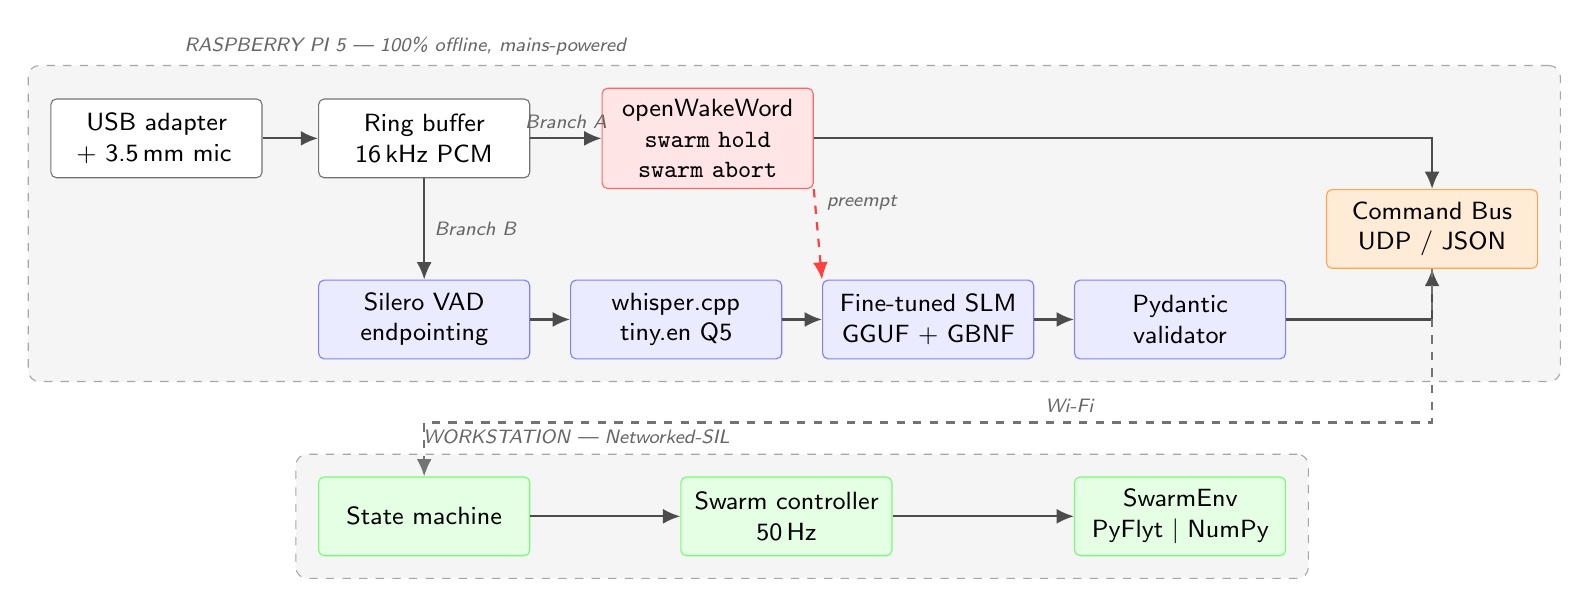
\begin{tikzpicture}[
  font=\sffamily\small,
  bx/.style   ={draw=black!55, rounded corners=2pt, align=center, inner sep=4pt,
                minimum height=10mm, fill=white, text width=24mm},
  reflex/.style={bx, fill=red!10,   draw=red!60},
  cortex/.style={bx, fill=blue!8,   draw=blue!50},
  ctrlb/.style ={bx, fill=green!10, draw=green!55},
  busb/.style  ={bx, fill=orange!16,draw=orange!70},
  ar/.style    ={-{Latex[length=2.2mm,width=1.9mm]}, thick, draw=black!70},
  arp/.style   ={ar, dashed, draw=red!75},
  arw/.style   ={ar, dashed, draw=black!55},
  lbl/.style   ={font=\sffamily\scriptsize\itshape, text=black!60},
]

% ---- Lane A : reflex (top) ----
\node[bx]     (mic) at ( 0.0, 4.3) {USB adapter\\ + 3.5\,mm mic};
\node[bx]     (buf) at ( 3.4, 4.3) {Ring buffer\\ 16\,kHz PCM};
\node[reflex] (oww) at ( 7.0, 4.3) {openWakeWord\\ \code{swarm hold}\\ \code{swarm abort}};

% ---- Lane B : cortex (middle) ----
\node[cortex] (vad) at ( 3.4, 2.0) {Silero VAD\\ endpointing};
\node[cortex] (stt) at ( 6.6, 2.0) {whisper.cpp\\ tiny.en Q5};
\node[cortex] (slm) at ( 9.8, 2.0) {Fine-tuned SLM\\ GGUF + GBNF};
\node[cortex] (val) at (13.0, 2.0) {Pydantic\\ validator};

% ---- Command bus ----
\node[busb]   (bus) at (16.2, 3.15) {Command Bus\\ UDP / JSON};

% ---- Workstation (bottom) ----
\node[ctrlb]  (sm)  at ( 3.4,-0.5) {State machine};
\node[ctrlb]  (ctl) at ( 8.0,-0.5) {Swarm controller\\ 50\,Hz};
\node[ctrlb]  (env) at (13.0,-0.5) {SwarmEnv\\ PyFlyt \textbar{} NumPy};

% ---- edges ----
\draw[ar] (mic) -- (buf);
\draw[ar] (buf) -- node[lbl,above]{Branch A} (oww);
\draw[ar] (buf) -- node[lbl,right]{Branch B} (vad);
\draw[ar] (vad) -- (stt);
\draw[ar] (stt) -- (slm);
\draw[ar] (slm) -- (val);
\draw[ar] (oww.east) -| (bus.north);
\draw[ar] (val.east) -| (bus.south);
\draw[arp] (oww.south east) -- node[lbl,above right,pos=0.35]{preempt} (slm.north west);
\draw[arw] (bus.south) -- ++(0,-1.95) -| node[lbl,above,pos=0.18]{Wi-Fi} (sm.north);
\draw[ar] (sm)  -- (ctl);
\draw[ar] (ctl) -- (env);

% ---- enclosures ----
\begin{scope}[on background layer]
  \node[draw=black!35, dashed, rounded corners=4pt, fill=black!4, inner sep=8pt,
        fit=(mic)(buf)(oww)(vad)(stt)(slm)(val)(bus),
        label={[lbl]above left:RASPBERRY PI 5 --- 100\% offline, mains-powered}] {};
  \node[draw=black!35, dashed, rounded corners=4pt, fill=black!4, inner sep=8pt,
        fit=(sm)(ctl)(env),
        label={[lbl]above left:WORKSTATION --- Networked-SIL}] {};
\end{scope}
\end{tikzpicture}}
\caption{Dual-path architecture. Branch A bypasses STT entirely to guarantee the safety-reflex budget;
Branch B performs full transcription and structured parsing. Physics simulation runs off-device.}
\label{fig:arch}
\end{figure}

Three architectural decisions are fixed here and not revisited.

\begin{enumerate}[leftmargin=1.6em,itemsep=4pt]
  \item \textbf{Physics runs off-device.} The claim under test is that \emph{perception and language
        understanding} fit on the edge device --- not that a PyBullet physics engine does. Co-locating them
        contends for cores and makes latency measurements irreproducible.
  \item \textbf{A minimal Command Bus, not a distributed middleware.} Roughly forty lines of UDP/JSON
        behind an abstract interface. A peer-to-peer mesh transport is the right \emph{eventual} answer and
        remains a one-file swap; adopting one now buys an entire failure class for no measurable result.
  \item \textbf{The schema is not in the prompt, and the static prefix is KV-cached.} Fine-tuning is
        precisely what removes the need to describe the schema at inference time. This holds per-command
        prefill at roughly 15 tokens instead of roughly 290 --- the difference between meeting and missing
        the latency target, and the reason \code{-c 512} is sufficient context.
\end{enumerate}

\subsection{Component inventory}

Table~\ref{tab:comp} is the build list. Every row is a module that must exist, with one responsibility and
one owner file.

\begin{longtable}{@{}P{0.18}P{0.20}P{0.20}P{0.30}@{}}
\caption{Component inventory}\label{tab:comp}\\
\toprule
\textbf{Component} & \textbf{Technology} & \textbf{Module} & \textbf{Responsibility} \\
\midrule
\endfirsthead
\multicolumn{4}{@{}l}{\small\itshape Table \thetable\ (continued)}\\
\toprule
\textbf{Component} & \textbf{Technology} & \textbf{Module} & \textbf{Responsibility} \\
\midrule
\endhead
\bottomrule
\endlastfoot
Audio capture & ALSA, \code{sounddevice} & \code{runtime/audio.py} & 48\munit{kHz} mono capture, ring
  buffer, resample to 16\munit{kHz}, timestamp every frame \\
Keyword spotter & openWakeWord ONNX & \code{runtime/branch\_a.py} & Two-class detection, threshold and
  smoothing, publish on trigger, raise the preempt flag \\
Endpointing & Silero VAD ONNX & \code{runtime/vad.py} & Detect speech onset and end-of-speech; emit the
  segment and the end-of-speech timestamp \\
Speech recognition & \code{whisper.cpp tiny.en} Q5 & \code{runtime/stt.py} & Segment $\rightarrow$
  transcript, \code{-t 3}, greedy \\
Command parser & \code{llama.cpp} + GBNF & \code{runtime/parser.py} & Transcript $\rightarrow$ JSON
  string, grammar-constrained, greedy, abortable \\
Validator (layer 2) & Pydantic v2 & \code{schema/validate.py} & Required slots, envelope clamps,
  identifier filtering, fallback to \code{HOVER} \\
Canonicaliser & Pure Python & \code{schema/canon.py} & The single comparison function used by every
  accuracy metric (\S\ref{sec:defs}) \\
State machine (layer 3) & Pure Python & \code{swarm/fsm.py} & Reject commands illegal in the current
  flight state; own the \code{ABORTED} recovery path \\
Command bus & UDP + JSON & \code{runtime/bus.py} & Publish and subscribe, monotonic sequence numbers,
  branch tag \\
Swarm controller & NumPy & \code{swarm/control.py} & Boids, formation slot assignment, APF separation,
  hard geometric clamp, PID point navigation, 50\munit{Hz} \\
Simulation backends & PyFlyt/PyBullet; NumPy & \code{swarm/env\_pyflyt.py},
  \code{swarm/env\_numpy.py} & Implement one \code{SwarmEnv} interface: \code{reset}, \code{step},
  \code{state} \\
Benchmark harness & Python, \code{psutil} & \code{eval/bench.py} & One CSV row per trial: accuracy,
  per-stage latency, peak RSS, temperature, throttle flags \\
\end{longtable}

\subsection{What Branch A carries --- and what it must not}
\label{sec:branchA}

Branch~A is always listening, so every keyword class is a permanent false-accept surface. Membership is
therefore decided by a rule, not by preference. A command belongs in Branch~A only if it satisfies
\textbf{both} tests:

\begin{enumerate}[leftmargin=1.6em,itemsep=3pt]
  \item \textbf{Latency-decisive.} The Branch~A/B delta changes the physical outcome. That delta is
        $2{,}500 - 150 = 2{,}350$\munit{ms}; at the validator's own \code{speed} ceiling of
        2.0\munit{m/s} it is \textbf{4.7\munit{m} of uncommanded travel} --- comparable to the full radius
        of the 1--10\munit{m} formation envelope. A drone can cross the formation before Branch~B answers.
  \item \textbf{Fail-safe under false accept.} An unprompted trigger must move the swarm \emph{toward}
        safety. Branch~A may only ever make the swarm do \emph{less}, never more.
\end{enumerate}

Table~\ref{tab:branchA} applies both tests to every intent in schema v1.0. Exactly two survive.

\begin{table}[htbp]
\centering
\caption{The membership rule applied to all ten intents. Exactly two qualify.}
\label{tab:branchA}
\small
\begin{tabular}{@{}P{0.20}P{0.24}P{0.22}P{0.16}@{}}
\toprule
\textbf{Intent} & \textbf{Latency-decisive?} & \textbf{Fail-safe?} & \textbf{Branch} \\
\midrule
\code{abort}      & Yes                              & Yes  & \textbf{A} \\
\code{hover}      & Yes                              & Yes  & \textbf{A} \\
\midrule
\code{land}       & No --- descent is itself slow    & Yes  & B \\
\code{set\_param} & No                               & Yes  & B \\
\code{unknown}    & No                               & Yes  & B \\
\midrule
\code{takeoff}    & ---                              & \textbf{No} --- spins up rotors & B only \\
\code{move}       & ---                              & \textbf{No} --- uncommanded manoeuvre & B only \\
\code{altitude}   & ---                              & \textbf{No} & B only \\
\code{rotate}     & ---                              & \textbf{No} & B only \\
\code{formation}  & ---                              & \textbf{No} & B only \\
\bottomrule
\end{tabular}
\end{table}

The two classes map onto intents that already exist in the schema, so Branch~A adds no grammar rule, no
schema field, and no controller entry point:

\begin{itemize}[leftmargin=1.4em,itemsep=3pt]
  \item \code{swarm hold} $\rightarrow$ \code{\{"intent":"hover"\}} --- stop lateral motion, hold current
        altitude, rotors running, \textbf{mission recoverable}. This is already the system's designated
        safe state: every validation failure, parse failure, and \code{max\_tokens} truncation resolves to
        it, so exposing it as a reflex makes the fallback state reachable at reflex speed.
  \item \code{swarm abort} $\rightarrow$ \code{\{"intent":"abort"\}} --- \textbf{immediate descent in
        place, motors off on ground contact.} Mission terminated, not recoverable by voice.
\end{itemize}

\begin{panel}
\textbf{Why \code{abort} is land-in-place and not disarm.} Three definitions were available: disarm
(motors off in flight), land in place, or return-to-launch. Disarm inside a $[0.5, 15]$\munit{m} altitude
envelope is a decision to destroy the airframe; return-to-launch requires \emph{flying}, which is the thing
being stopped. Land-in-place removes energy from the situation with no lateral motion. It is also what
makes the two reflex classes semantically disjoint: \code{hold} stays up, \code{abort} comes down.

\textbf{Why a three-syllable phrase, and why a shared prefix is safe.} A bare monosyllable is the worst
case for always-on spotting: the classifier head sees a fixed embedding window of over a second, so a
300\munit{ms} word supplies little discriminative signal and false accepts on continuous speech rise
accordingly. The \code{swarm} prefix contributes an acoustically uncommon /sw/ onset to both classes at
once. The shared prefix does reduce inter-class margin --- but \textbf{both off-diagonal cells of the
confusion matrix are fail-safe}: hearing \code{abort} for \code{hold} is strictly more conservative, and
the reverse is still a stop. Confusion \emph{within} a fail-safe set is a benign error class, which is
precisely what test~2 buys.

\textbf{Deliberately excluded: \code{resume}.} The obvious third class, and the most dangerous. A false
accept would restart motion in a situation the operator deliberately froze --- it would undo a safety
action. Resume is reachable only through Branch~B, where the 2.35\munit{s} delay costs nothing.
\end{panel}

\subsection{Preemption mechanism}

When Branch~A triggers while Branch~B is mid-inference, two things must happen, and only one of them is a
correctness requirement.

\begin{itemize}[leftmargin=1.4em,itemsep=3pt]
  \item \textbf{Correctness (mandatory).} Every bus message carries a monotonically increasing sequence
        number and a \code{branch} tag. The state machine discards any Branch~B message whose sequence
        number is lower than the highest Branch~A message already applied. A stale Branch~B result
        therefore \emph{cannot} take effect, whether or not its decode was stopped.
  \item \textbf{Optimisation (desirable).} Abort the in-flight decode so the three inference cores are
        released immediately. Spike~S7 establishes whether the chosen \code{llama.cpp} binding supports
        this. If it does not, the SLM runs in a separate process that can be signalled, and the sequence
        rule alone carries correctness.
\end{itemize}

NFR-17 bounds the recovery: the time from a Branch~A trigger until Branch~B can accept a new utterance.

\subsection{Latency budget}

\begin{table}[htbp]
\centering
\caption{Latency budget. These are targets; measured p95 values from Exp-2 replace them.}
\label{tab:latency}
\small
\begin{tabular}{@{}P{0.62}P{0.20}@{}}
\toprule
\textbf{Stage} & \textbf{Target p95} \\
\midrule
VAD endpointing (wall-clock wait to confirm end of speech)   & 500\munit{ms} \\
STT (\code{whisper.cpp tiny.en} Q5, \code{-t 3})             & 1{,}200\munit{ms} \\
SLM prefill (cached prefix, $\approx$15 tokens)              & 250\munit{ms} \\
SLM decode ($\approx$22 tokens, null-omitting schema)        & 1{,}100\munit{ms} \\
Validate, state-machine check, and dispatch                  & 50\munit{ms} \\
\midrule
\textbf{E2E from end-of-speech (headline)}                    & \textbf{$\leq$ 2{,}500\munit{ms}} \\
E2E from start-of-speech (3\munit{s} utterance)               & $\leq$ 5{,}500\munit{ms} \\
\textbf{Branch A reflex, from keyword \emph{offset}} (headline) & \textbf{$\leq$ 150\munit{ms}} \\
Branch A reflex, from keyword \emph{onset} ($\approx$700\munit{ms} phrase) & $\leq$ 850\munit{ms} \\
\bottomrule
\end{tabular}
\end{table}

Both anchors are reported, for both branches. Reporting only end-of-speech looks evasive; reporting only
start-of-speech penalises the system for the length of the operator's sentence.

The headline Branch~A figure anchors at keyword \emph{offset} --- the last frame of the phrase in the ring
buffer. An onset-anchored target of 150\munit{ms} is unsatisfiable by construction, because a
$\approx$700\munit{ms} phrase cannot be classified before it has been heard; the floor on an onset-anchored
measurement is the utterance duration itself. Offset anchoring isolates system compute --- melspectrogram,
shared speech embedding, classifier head, bus publish, plus frame quantisation and the activation-smoothing
window --- exactly as the end-of-speech anchor does for Branch~B. The onset figure is reported alongside as
operator-perceived reflex time, which also exposes the real trade in phrase choice: roughly
150\munit{ms} of perceived reflex per additional syllable, bought in exchange for a lower false-accept
rate.

\subsection{CPU core allocation}

The Pi 5 has four Cortex-A76 cores. Branch~A must never be starved by Branch~B, because NFR-1 has to hold
\emph{while} the SLM is decoding --- which is exactly the second condition Exp-2 measures.

\begin{table}[htbp]
\centering
\caption{Core allocation, pinned with \code{taskset} and verified during Exp-1 and Exp-2}
\label{tab:cores}
\small
\begin{tabular}{@{}P{0.10}P{0.45}P{0.35}@{}}
\toprule
\textbf{Core} & \textbf{Assignment} & \textbf{Verification} \\
\midrule
0     & ALSA capture thread, ring buffer, Silero VAD, openWakeWord (Branch A) &
  \code{taskset -c 0}; per-frame spotter compute must stay under the frame period, logged every frame \\
1--3  & \code{whisper.cpp -t 3} and \code{llama.cpp -t 3} --- never concurrent, so they share the same
  three cores without contention &
  \code{taskset -c 1-3}; \code{htop} during Exp-1; tokens/s compared against spike S1 \\
\bottomrule
\end{tabular}
\end{table}

STT and the SLM are sequential by construction: the parser cannot start before the transcript exists.
That is what makes a three-core allocation sufficient for both.

\subsection{Memory budget}

Table~\ref{tab:mem} computes the worst-case resident set from parameter counts and bits per weight, so
NFR-9a is a checkable arithmetic claim rather than a hope. Q8\_0 costs approximately 8.5 bits per weight
and Q4\_K\_M approximately 4.85.

\begin{table}[htbp]
\centering
\caption{Worst-case memory budget --- Llama-3.2-1B at Q8\_0, the largest of the six configurations}
\label{tab:mem}
\small
\begin{tabular}{@{}P{0.40}P{0.18}P{0.30}@{}}
\toprule
\textbf{Component} & \textbf{Peak RSS} & \textbf{Basis} \\
\midrule
SLM weights            & 1.32\munit{GB} & 1.24\munit{B} parameters at 8.5 bits per weight \\
KV cache               & 0.10\munit{GB} & \code{-c 512}; actual context is $\approx$40 tokens \\
\code{whisper.cpp} \code{tiny.en} Q5 & 0.08\munit{GB} & 39\munit{M} parameters plus mel buffers \\
openWakeWord           & 0.10\munit{GB} & Melspectrogram and shared embedding models plus two heads \\
Python, NumPy, ONNX Runtime & 0.35\munit{GB} & Interpreter and native libraries \\
\midrule
\textbf{Worst case, full stack} & \textbf{1.93\munit{GB}} & Sum of the above \\
Lightest configuration (SmolLM2-360M Q4\_K\_M) & $\approx$0.85\munit{GB} & 0.22\munit{GB} of weights plus
  the same fixed 0.63\munit{GB} \\
\bottomrule
\end{tabular}
\end{table}

Against 8\munit{GB} of physical memory, all six configurations fit with large headroom. Memory is
therefore a \emph{reported} quantity for RQ1, not a live risk --- NFR-9b --- with a single pass/fail cap on
the selected deployment configuration in NFR-9a.

\subsection{Audio paths}
\label{sec:audio}

Two paths exist and must not be confused, because one of them is allowed to be slow.

\begin{itemize}[leftmargin=1.4em,itemsep=3pt]
  \item \textbf{Corpus path (offline, quality-first).} Capture at 48\munit{kHz}, \code{S16\_LE}, mono, to
        WAV. Resample 3:1 to 16\munit{kHz} offline with \code{soxr} at very-high quality. \textbf{Never}
        ALSA \code{plug} resampling for corpus audio: its quality is unspecified and it would silently
        become an uncontrolled variable in Exp-3.
  \item \textbf{Live path (online, latency-first).} Either capture 16\munit{kHz} directly if the adapter
        supports it natively, or resample online with one fixed polyphase filter whose cost is measured.
        The choice is made at spike~S0 and written into the spike report.
\end{itemize}

$T_0$ for Branch~B is the timestamp of the last PCM frame present in the ring buffer at the moment the VAD
declares end-of-speech. Capture and buffering latency sits \emph{before} $T_0$; it is measured once at S0
with a loopback test and reported as a separate number rather than folded into Table~\ref{tab:latency}.
The Wi-Fi hop from the Pi to the workstation is likewise measured once with a UDP echo and reported as a
single figure, because it sits after dispatch and is not part of the perception budget.

% =====================================================================
\section{Command schema v1.0 and the three validation layers}
\label{sec:schema}

Frozen on \textbf{D1}, before any data generation. Ten intents: \code{formation}, \code{move},
\code{altitude}, \code{takeoff}, \code{land}, \code{hover}, \code{abort}, \code{rotate},
\code{set\_param}, \code{unknown}.

\begin{lstlisting}[caption={Wire format --- single-line JSON, fixed key order, null fields omitted},captionpos=b]
{"intent":"formation","shape":"circle","radius":5.0}
{"intent":"move","pos":[10.0,0.0,3.0],"speed":1.5}
{"intent":"move","dir":"north","dist":10.0}
{"intent":"altitude","z":4.0,"ids":[1,2]}
{"intent":"rotate","yaw":90.0}
{"intent":"set_param","speed":1.0}
{"intent":"hover"}
{"intent":"abort"}
{"intent":"unknown"}
\end{lstlisting}

Omitting null fields rather than emitting them explicitly cuts a typical command from roughly 40 tokens to
about 18 --- at Pi 5 decode rates, close to a full second of latency per command, recovered for free. This
is the second-largest latency win in the project after keeping the schema out of the prompt.

\subsection{Layer 1 --- GBNF grammar: guarantees structure}

\begin{lstlisting}[caption={cmd.gbnf --- the grammar that constrains decoding},captionpos=b]
root      ::= cmd
cmd       ::= c-form | c-move | c-alt | c-takeoff | c-land | c-hover
            | c-abort | c-rot | c-param | c-unk

c-form    ::= "{\"intent\":\"formation\",\"shape\":" shape o-radius o-spacing o-ids "}"
c-move    ::= "{\"intent\":\"move\","  ( kv-pos | kv-dir ) o-speed o-ids "}"
c-alt     ::= "{\"intent\":\"altitude\",\"z\":" num o-ids "}"
c-takeoff ::= "{\"intent\":\"takeoff\""  o-z o-ids "}"
c-land    ::= "{\"intent\":\"land\""     o-ids "}"
c-hover   ::= "{\"intent\":\"hover\""    o-ids "}"
c-abort   ::= "{\"intent\":\"abort\"}"
c-rot     ::= "{\"intent\":\"rotate\",\"yaw\":" num o-ids "}"
c-param   ::= "{\"intent\":\"set_param\"" o-speed o-spacing o-alt "}"
c-unk     ::= "{\"intent\":\"unknown\"}"

shape     ::= "\"circle\"" | "\"line\"" | "\"wedge\"" | "\"grid\""
            | "\"column\"" | "\"flock\""
dir       ::= "\"north\"" | "\"south\"" | "\"east\"" | "\"west\"" | "\"up\""
            | "\"down\"" | "\"forward\"" | "\"back\"" | "\"left\"" | "\"right\""

kv-pos    ::= "\"pos\":[" num "," num "," num "]"
kv-dir    ::= "\"dir\":" dir ",\"dist\":" num

o-radius  ::= ( ",\"radius\":"  num )?
o-spacing ::= ( ",\"spacing\":" num )?
o-speed   ::= ( ",\"speed\":"   num )?
o-alt     ::= ( ",\"alt\":"     num )?
o-z       ::= ( ",\"z\":"       num )?
o-ids     ::= ( ",\"ids\":[" idlist "]" )?
idlist    ::= [0-9] ( "," [0-9] )*

num       ::= "-"? [0-9] [0-9]? [0-9]? ( "." [0-9] )?
\end{lstlisting}

The \code{num} rule caps values at three integer digits plus one decimal. This is what structurally
prevents \code{1e999}, twenty-digit integers, and a bare \code{2.}\ from ever being emitted. \textbf{GBNF
cannot express numeric ranges}, only digit counts --- range enforcement belongs to layer 2. The one-decimal
limit is also why the comparator in \S\ref{sec:defs} rounds to one decimal: the metric matches what the
decoder can produce.

\subsection{Layer 2 --- semantic validator: guarantees meaning}

\begin{itemize}[leftmargin=1.4em,itemsep=2pt]
  \item \textbf{Required-slot matrix.} \code{formation} requires \code{shape}; \code{circle} requires
        \code{radius}; \code{line}, \code{grid}, and \code{column} require \code{spacing};
        \code{altitude} requires \code{z}; \code{move} requires exactly one of \code{pos} or
        (\code{dir} + \code{dist}); \code{rotate} requires \code{yaw}; \code{set\_param} requires at
        least one slot.
  \item \textbf{Physical envelope --- clamp and log, never reject.}
        \code{radius} $\in [1,10]$\munit{m}; \code{spacing} $\in [1,5]$\munit{m};
        \code{z} $\in [0.5,15]$\munit{m}; \code{speed} $\in [0.2,2.0]$\munit{m/s};
        $|\code{pos}| \leq 50$\munit{m}; \code{yaw} $\in [-180,180]^{\circ}$. A clamped command is safer
        than a dropped one.
  \item \textbf{Identifier handling.} \code{ids} $\subseteq \{0 \dots N{-}1\}$; out-of-range identifiers
        are dropped with a log line; the list is \textbf{deduplicated and sorted ascending}; empty after
        filtering means all drones. Duplicate identifiers are in the adversarial test corpus.
  \item \textbf{Fallback.} Any validation failure, parse failure, or \code{max\_tokens} truncation
        resolves to \code{HOVER} plus a structured log entry. Never to a movement command.
\end{itemize}

\subsection{Layer 3 --- flight state machine: guarantees legality}

A command can be well-formed and physically sensible and still be wrong for the current state: \code{move}
while landed, \code{takeoff} while already flying. Layer 3 rejects those before dispatch.

States are \code{LANDED}, \code{TAKING\_OFF}, \code{FLYING}, \code{LANDING}, \code{ABORTED}. Transitions:
\code{LANDED} $\rightarrow$ \code{TAKING\_OFF} on \code{takeoff}; \code{TAKING\_OFF} $\rightarrow$
\code{FLYING} when the target altitude is reached; \code{FLYING} $\rightarrow$ \code{LANDING} on
\code{land}; \code{LANDING} $\rightarrow$ \code{LANDED} on ground contact; and \code{abort} from any
airborne state $\rightarrow$ \code{ABORTED}.

\begin{table}[htbp]
\centering
\caption{Command legality by flight state. Rejections resolve to \code{HOVER} with a log entry.}
\label{tab:states}
\small
\begin{tabular}{@{}P{0.20}P{0.36}P{0.34}@{}}
\toprule
\textbf{Intent} & \textbf{Legal in} & \textbf{Rejected in} \\
\midrule
\code{takeoff}   & \code{LANDED} & \code{TAKING\_OFF}, \code{FLYING}, \code{LANDING}, \code{ABORTED} \\
\code{land}      & \code{TAKING\_OFF}, \code{FLYING} & \code{LANDED}, \code{LANDING}, \code{ABORTED} \\
\code{hover}     & \code{TAKING\_OFF}, \code{FLYING} & \code{LANDED}, \code{LANDING}, \code{ABORTED} \\
\code{abort}     & \code{TAKING\_OFF}, \code{FLYING}, \code{LANDING} & \code{LANDED}, \code{ABORTED}
  --- accepted as a logged no-op, never an error \\
\code{move}, \code{altitude}, \code{rotate}, \code{formation} & \code{FLYING} & every other state \\
\code{set\_param} & every state except \code{ABORTED} & \code{ABORTED} \\
\code{unknown}   & --- & never dispatched; logged only \\
\bottomrule
\end{tabular}
\end{table}

\textbf{Recovery from \code{ABORTED}.} Because \code{resume} is deliberately absent from the vocabulary,
\code{ABORTED} would otherwise be a dead end --- and a dead end on camera during the demonstration.
Recovery is explicit, manual, and non-vocal: the operator runs \code{./run\_pipeline.sh -{}-reset}, which
re-initialises the state machine to \code{LANDED} only after every drone reports ground contact and
near-zero velocity, and writes a reset record to the log. Recovery is never reachable by speech, which is
what keeps the reflex one-directional.

% =====================================================================
\section{Definitions of record}
\label{sec:defs}

Every accuracy number in either thesis comes from the functions defined here. They are frozen on D1
alongside the schema, because a metric changed after results exist is not a metric.

\subsection{Canonical form and the single comparator}

\code{schema/canon.py} exposes one function, \code{canon(obj)}, applied to \emph{both} the prediction and
the reference before any comparison:

\begin{enumerate}[leftmargin=1.6em,itemsep=2pt,topsep=3pt]
  \item Key order fixed by schema declaration order.
  \item Absent and null fields omitted, not emitted.
  \item Floats rounded to \textbf{one decimal} --- matching the \code{num} rule's precision limit.
  \item \code{ids} deduplicated and sorted ascending.
  \item No whitespace outside string literals.
\end{enumerate}

Two commands are equal if and only if their canonical forms are byte-identical; numeric slots are equal if
and only if $\mathrm{round}(a,1) = \mathrm{round}(b,1)$.

\textbf{Exact match and command recognition rate use this same comparator.} They differ in exactly two
respects: the input modality (reference text for EM, audio for CRR) and the measurement point. That is
deliberate --- it makes the difference between them attributable to a single cause.

\begin{panel}
\textbf{Why EM minus CRR is itself a result.} Exp-1 feeds \emph{reference text} to the parser, so the
model is the only variable and the three models can be separated from one another. Exp-3 feeds
\emph{audio} through the whole pipeline. Because the comparator is identical, the gap between the two
numbers on the same items is the \textbf{cost of the speech-recognition stage}, and it is reported as a
finding rather than absorbed into a single end-to-end score. Feeding audio to Exp-1 would impose a word
error rate ceiling on all three models at once, squeezing them together and making any remaining
difference unattributable.
\end{panel}

\subsection{Metric definitions}

Table~\ref{tab:defs} fixes each metric and names the experiment it feeds. A metric absent from this table
does not appear in either thesis.

\begin{table}[htbp]
\centering
\caption{Metric definitions of record}
\label{tab:defs}
\small
\begin{tabular}{@{}P{0.16}P{0.44}P{0.30}@{}}
\toprule
\textbf{Metric} & \textbf{Definition} & \textbf{Used in} \\
\midrule
Exact match (EM) & Fraction of items where \code{canon(pred)} equals \code{canon(gold)}. Input is
  \textbf{reference text}. & Exp-1, NFR-4 \\
Command recognition rate (CRR) & The same comparison, with input being \textbf{audio} through the full
  pipeline. & Exp-3, NFR-7, NFR-8 \\
Intent macro-F1 & Unweighted mean of per-intent F1 over all ten intents present in the reference. Macro,
  so \code{unknown} cannot be inflated by frequency. & Exp-1, NFR-5 \\
Slot-F1 & Micro-averaged F1 over the multiset of \code{(key, canonical value)} pairs, across all items
  regardless of intent correctness. & Exp-1 \\
Safe-failure rate & Among items where EM is 0, the fraction whose dispatched action is \code{unknown} or
  \code{HOVER}. \textbf{Denominator is failed items only.} Always reported next to EM or CRR, because a
  model that always emits \code{hover} scores 1.0 here and near-zero on EM. & Exp-1, Exp-3, NFR-9 \\
False-command rate & On the out-of-domain set, the fraction of items producing any intent other than
  \code{unknown} that also survives the validator. & Exp-1, NFR-18 \\
Word error rate (WER) & Standard word-level edit distance after a fixed normalisation: lowercase,
  punctuation stripped, digits expanded via the mapping committed in \code{eval/norm.py}. & Exp-0, Exp-3 \\
Latency & Branch~B: $T_0$ = end-of-speech, $T_1$ = return of the bus publish call. Branch~A: $T_0$ =
  keyword offset, same $T_1$. Both branches additionally report an onset-anchored figure. & Exp-2 \\
Percentiles & Nearest-rank on the sorted sample, no interpolation. The sample size $n$ is stated in every
  cell. & Exp-1, Exp-2, Exp-3 \\
Formation accuracy (FA) & Fraction of drones within $\tau = 0.5$\munit{m} of the assigned slot, averaged
  over the final 5\munit{s} of a 60\munit{s} trial. & Exp-4, NFR-13 \\
Convergence & Rate of trials reaching FA $\geq 0.85$ at all, plus median and IQR of convergence time
  \emph{over converged trials only}. & Exp-4 \\
\bottomrule
\end{tabular}
\end{table}

\begin{panel}
\textbf{Accuracy $n$ and latency $n$ are different numbers.} Decoding is greedy under a fixed grammar, so
the model's output for a given input is deterministic. One pass over a test set therefore establishes
accuracy exactly, and $n_{\mathrm{accuracy}}$ equals the number of test items. Latency is not
deterministic --- it varies with scheduling, cache state, and temperature --- so
$n_{\mathrm{latency}}$ equals the number of timed repetitions, fixed at 200 per configuration. Reporting
one $n$ for both would be wrong in one direction or the other.
\end{panel}

% =====================================================================
\section{Functional requirements}

Every requirement in Table~\ref{tab:fr} carries its own verification method; a requirement with no stated
way to check it is not a requirement.

\begin{longtable}{@{}P{0.07}P{0.62}P{0.24}@{}}
\caption{Functional requirements}\label{tab:fr}\\
\toprule
\textbf{ID} & \textbf{Requirement} & \textbf{Verification} \\
\midrule
\endfirsthead
\multicolumn{3}{@{}l}{\small\itshape Table \thetable\ (continued)}\\
\toprule
\textbf{ID} & \textbf{Requirement} & \textbf{Verification} \\
\midrule
\endhead
\bottomrule
\endlastfoot
\textbf{FR-1}  & Publish a reproducible dataset (\S\ref{sec:data}): $\approx$2{,}400 synthetic
                 text--JSON pairs by label-first generation, a 320-file single-speaker golden set,
                 $\approx$150 out-of-domain examples, a two-class wake-word corpus, and a dataset card.
                 Splits assigned by \textbf{template family}, not by row. & Dataset card;
                 \code{check\_leakage.py}; every label accepted by \code{cmd.gbnf} \\
\textbf{FR-2}  & Fine-tune \textbf{three} SLMs (Qwen2.5-0.5B, SmolLM2-360M, Llama-3.2-1B) with an
                 identical LoRA recipe, identical data, and identical seed (\S\ref{sec:model}).
                 Completion-only loss masking. & Three adapters plus training logs \\
\textbf{FR-3}  & Export each to GGUF at \textbf{Q8\_0 and Q4\_K\_M} --- six artefacts --- and verify
                 HuggingFace$\leftrightarrow$\code{llama.cpp} tokenisation and chat-template parity on ten
                 fixed prompts. & \code{test\_template\_parity.py} green \\
\textbf{FR-4}  & Constrain all generative inference with the GBNF grammar; validate all output through the
                 Pydantic semantic validator. & \code{test\_grammar.py} including an adversarial corpus \\
\textbf{FR-5}  & Run STT offline on-device via \code{whisper.cpp tiny.en}; no network access at any point
                 in the pipeline. & End-to-end run with networking disabled \\
\textbf{FR-6}  & Implement Branch A: \textbf{two} fail-safe keyword classes ---
                 \code{swarm hold}$\rightarrow$\code{hover} and
                 \code{swarm abort}$\rightarrow$\code{abort} (\S\ref{sec:branchA}) --- either of which
                 \textbf{preempts} an in-flight Branch B inference by the sequence-number rule. No movement
                 verb may be added to Branch A. & Exp-2 preemption trials; 2$\times$2 cross-trigger
                 matrix \\
\textbf{FR-7}  & Implement the swarm controller: NumPy-vectorised Boids, formation slot assignment
                 (circle, line, wedge), APF separation with a hard geometric clamp at the integrator, and
                 PID point navigation; $N=5$, 50\munit{Hz}, against an abstract \code{SwarmEnv}. & Exp-4 \\
\textbf{FR-8}  & Provide two \code{SwarmEnv} backends: PyFlyt (primary) and a NumPy kinematic simulator
                 (fast iteration). & Both pass a hover smoke test \\
\textbf{FR-9}  & Run the full pipeline end to end from the live microphone for the demonstration. &
                 Demo video, networking disabled on camera \\
\textbf{FR-10} & Emit one CSV row per benchmark trial covering accuracy, per-stage latency, peak RSS,
                 temperature, and throttle flags. Every table and figure in both theses derives from these
                 CSVs. & \code{results/*.csv} committed \\
\textbf{FR-11} & Implement the flight state machine as validation layer 3, including the explicit
                 non-vocal recovery path out of \code{ABORTED} (\S\ref{sec:schema}). &
                 \code{test\_fsm.py} covering every cell of Table~\ref{tab:states} \\
\textbf{FR-12} & Implement the canonicaliser and the single comparator used by every accuracy metric
                 (\S\ref{sec:defs}). & \code{test\_canon.py}; EM and CRR call the same function \\
\end{longtable}

% =====================================================================
\section{Non-functional requirements}

Table~\ref{tab:nfr} states each target as a number a script can check, and names the experiment that
produces it.

\begin{longtable}{@{}P{0.07}P{0.47}P{0.24}P{0.11}@{}}
\caption{Non-functional requirements}\label{tab:nfr}\\
\toprule
\textbf{ID} & \textbf{Requirement} & \textbf{Target} & \textbf{Source} \\
\midrule
\endfirsthead
\multicolumn{4}{@{}l}{\small\itshape Table \thetable\ (continued)}\\
\toprule
\textbf{ID} & \textbf{Requirement} & \textbf{Target} & \textbf{Source} \\
\midrule
\endhead
\bottomrule
\endlastfoot
\textbf{NFR-1}   & Reflex latency (Branch A), from \textbf{keyword offset}, measured both idle and under
                   active Branch B inference & p95 $\leq$ 150\munit{ms} & Exp-2 \\
\textbf{NFR-2}   & Branch B latency, from end-of-speech & p95 $\leq$ 2{,}500\munit{ms} & Exp-2 \\
\textbf{NFR-3}   & Per-stage latency instrumented and reported against Table~\ref{tab:latency} &
                   Every stage, p50/p95/p99 & Exp-2 \\
\textbf{NFR-4}   & Exact match on the deployed quantised artefact, best model & $\geq$ 0.85 & Exp-1 \\
\textbf{NFR-5}   & Intent macro-F1, best model & $\geq$ 0.90 & Exp-1 \\
\textbf{NFR-6}   & Schema validity under GBNF & 100\% \emph{by construction} --- reported as a structural
                   guarantee, not an achievement & Exp-1 \\
\textbf{NFR-7}   & CRR on the golden set, clean audio & $\geq$ 0.80 & Exp-3 \\
\textbf{NFR-8}   & CRR at 10\munit{dB} SNR & $\geq$ 0.65 & Exp-3 \\
\textbf{NFR-9}   & Safe-failure rate --- proportion of errors resolving to \code{unknown} or \code{HOVER}
                   rather than a wrong action & $\geq$ 0.70 & Exp-1, Exp-3 \\
\textbf{NFR-9a}  & Peak resident memory, \emph{selected deployment configuration}, full stack &
                   $\leq$ 2.5\munit{GB} & Exp-1 \\
\textbf{NFR-9b}  & Peak resident memory, every configuration & Reported per configuration as an RQ1
                   result; no pass/fail & Exp-1 \\
\textbf{NFR-10}  & Thermal --- proportion of trials with a non-zero throttle flag & $\leq$ 5\%, and always
                   reported & Exp-1 \\
\textbf{NFR-11}  & Word error rate of \code{tiny.en} on the author's speech, positioned against a
                   multi-speaker distribution & Reported with a bootstrap 95\% CI & Exp-0 \\
\textbf{NFR-12}  & Inter-drone collisions & \textbf{zero observed} across all trials, with a hard
                   geometric separation clamp at the integrator & Exp-4 \\
\textbf{NFR-13}  & Formation accuracy: fraction of drones within $\tau = 0.5$\munit{m} of the assigned
                   slot over the final 5\munit{s} of a 60\munit{s} trial & $\geq$ 0.85 & Exp-4 \\
\textbf{NFR-14}  & Offline operation & 100\%, no network dependency & FR-5 \\
\textbf{NFR-15}  & Keyword false accepts, aggregate over both Branch A classes, on ambient-speech
                   negatives & $\leq$ 1 per hour & Exp-2 \\
\textbf{NFR-16}  & Keyword false rejects per class at the selected operating point & $\leq$ 0.10 &
                   Exp-2 \\
\textbf{NFR-17}  & Preemption recovery --- time from a Branch A trigger until Branch B can accept a new
                   utterance & p95 $\leq$ 300\munit{ms} & Exp-2 \\
\textbf{NFR-18}  & False-command rate on the out-of-domain set & $\leq$ 0.05 & Exp-1 \\
\textbf{NFR-19}  & Reproducibility: all dependencies pinned (PyFlyt version, \code{llama.cpp} commit SHA),
                   fixed seeds, one-command rerun & \code{requirements.txt}, \code{run\_all.sh} & --- \\
\end{longtable}

\begin{panel}
\textbf{On NFR-12.} The claim is ``zero collisions \emph{observed}'', backed by a geometric separation
clamp --- \textbf{not} ``zero collisions guaranteed by APF''. Artificial potential fields provide no such
guarantee: with discrete timesteps and bounded actuation, penetration is always possible, and APF has
well-known failure modes including local minima and oscillation. Claiming a guarantee invites a question
that cannot be answered.

\textbf{On NFR-15 and NFR-16.} These are not independent claims but a single \emph{operating point}
selected from the measured ROC in Exp-2. A detection threshold trades one against the other, so both must
be quoted together or neither is meaningful. Report the full per-class curve and mark the chosen threshold.
\end{panel}

% =====================================================================
\section{Dataset specification}
\label{sec:data}

Table~\ref{tab:dataset} lists every artefact the dataset consists of. Each row is a file that must exist,
with a role that explains why it exists; nothing is collected without a stated consumer.

\begin{longtable}{@{}P{0.20}P{0.14}P{0.24}P{0.30}@{}}
\caption{Dataset components}\label{tab:dataset}\\
\toprule
\textbf{Split} & \textbf{Size} & \textbf{Source} & \textbf{Role} \\
\midrule
\endfirsthead
\multicolumn{4}{@{}l}{\small\itshape Table \thetable\ (continued)}\\
\toprule
\textbf{Split} & \textbf{Size} & \textbf{Source} & \textbf{Role} \\
\midrule
\endhead
\bottomrule
\endlastfoot
\code{train\_synth} & $\approx$1{,}900 pairs & Label-first synthetic generation plus round-trip
  augmentation & LoRA fine-tuning \\
\code{val\_synth} & $\approx$250 pairs & Held-out template families & Checkpoint selection on exact
  match \\
\code{test\_synth} & $\approx$250 pairs & Held-out template families & Statistical power for Exp-1; the
  paired sample McNemar operates on \\
\code{test\_golden} & 320 audio files, 200 unique transcripts & Author, three recording sessions &
  Headline accuracy (transcripts) and all of Exp-3 (audio) \\
\code{test\_ood} & $\approx$150 items & Out-of-domain speech and adversarial phrasings & NFR-18
  false-command rate; the \code{unknown} intent's real test \\
\code{wake\_pos} & $\approx$1{,}500 clips per class & Piper TTS \cite{piper} through openWakeWord's
  official pipeline, with RIR and noise augmentation & Branch A training; evaluated by limited-vocabulary
  keyword-spotting practice \cite{speechcmd} \\
\code{wake\_neg} & $\geq$ 3\munit{h} & Ambient speech, podcasts, and room noise & NFR-15 false-accept
  measurement; the denominator behind ``per hour'' \\
\code{commonvoice} & 300 clips & Mozilla Common Voice English, validated \cite{commonvoice} & Exp-0
  speaker-sensitivity baseline \\
\end{longtable}

\subsection{Synthetic generation --- label first}

Generation runs \textbf{label first}: write the target JSON, then request eight natural phrasings of it.
The reverse order --- write sentences, then label them --- reintroduces the annotation cost that generation
was supposed to remove, and produces label noise. Diversity axes are enumerated explicitly rather than
left to sampling temperature: imperative and polite forms, unit variants (metres, m), numeric forms (five,
5, 5.0), drone subsetting (all, drone two, drones one and three), synonym sets per intent, filler words,
self-corrections, and truncated utterances.

Splits are assigned by \textbf{template family}: every paraphrase descended from one label lands in the
same split. Row-wise splitting would put near-duplicates on both sides of the boundary and inflate every
accuracy figure. \code{check\_leakage.py} enforces this and is a gate, not a report.

\textbf{Conformance assert.} Every label in every split must be accepted by \code{cmd.gbnf}. A label the
grammar cannot produce is an unreachable target that silently caps accuracy. This assert is part of the
D1 gate and runs again after every regeneration.

\subsection{Audio: TTS bulk plus a single-speaker golden set}

Bulk audio is Piper TTS mixed with noise at four SNR levels and passed back through \code{whisper.cpp} for
\textbf{round-trip augmentation}, so the training data contains the transcription errors the model will
actually face at inference time.

The golden set is \textbf{one speaker --- the author --- in 320 files}:

\begin{itemize}[leftmargin=1.4em,itemsep=2pt]
  \item \textbf{Session 1:} 200 utterances, quiet room, covering all ten intents and every slot
        combination in the required-slot matrix.
  \item \textbf{Session 2:} a 60-utterance subset in a different room with real background --- corridor
        noise, fan, distant conversation.
  \item \textbf{Session 3:} the same 60-utterance subset on a different day, capturing day-to-day voice
        variation and microphone placement.
\end{itemize}

SNR levels for Exp-3 are mixed \emph{digitally} from session 1's clean audio, so no level requires
re-recording. \textbf{This is not a speaker-independence claim and is never presented as one.} Holding the
speaker fixed is an internal-validity choice: in Exp-3 it makes noise the only varying factor, which is
what licenses the causal statement about SNR. External validity across speakers is recovered where it
actually matters --- at the acoustic model --- by Exp-0. The parser stage consumes text and is
speaker-invariant by construction, so a multi-speaker corpus would add nothing to RQ1.

\subsection{Noise, SNR, and annotation agreement}

The noise corpus is named explicitly in the dataset card with its licence and URL: ESC-50
\cite{esc50} for environmental classes and DREGON \cite{dregon} for UAV-embedded rotor noise. SNR is
defined on \textbf{active-speech level} against noise RMS, not full-file RMS --- full-file RMS would let
leading silence set the level and make nominal SNR depend on how promptly the speaker started.
\code{data/mix\_noise.py} is committed, seeded, and is the only path by which noisy audio is produced.

Annotation agreement is measured on \textbf{50 golden-set utterances} by \textbf{test--retest with a single
annotator}: the author labels the 50 items against the schema at D5, seals that pass, then relabels the
same items cold at D15 --- a gap of ten days --- and the two passes are compared. This is
\textbf{intra}-annotator agreement and is reported as such. It establishes that the schema is applied
\emph{stably}; it does not establish that a second reader would apply it the same way, which is a strictly
stronger claim and is not made anywhere. Disagreements between the passes are the useful output: each one
localises an ambiguity in the schema or in the required-slot matrix.

Pass 1 remains the authoritative gold label, because the dataset freezes at D5. The D15 pass is a
measurement of consistency, not a revision --- consistent with R-4, a schema gap found after the freeze is
recorded as future work and does not trigger regeneration.

Synthetic labels need no annotation at all: they are generated label-first, so the label is the source
rather than a judgement. The 50 golden-set items are the only place in the entire project where annotation
occurs.

The negative corpus behind NFR-15 is \textbf{at least three hours}, and the false-accept figure is reported
as a count per hour \emph{with a Poisson confidence interval}. ``Zero false accepts'' over three hours is
consistent with a true rate near one per hour; stating the interval is what keeps the claim honest.

% =====================================================================
\section{Model pipeline}
\label{sec:model}

\begin{table}[htbp]
\centering
\caption{Fine-tuning recipe --- identical across all three models}
\label{tab:lora}
\small
\begin{tabular}{@{}P{0.34}P{0.56}@{}}
\toprule
\textbf{Setting} & \textbf{Value} \\
\midrule
Base models          & Qwen2.5-0.5B-Instruct, SmolLM2-360M-Instruct, Llama-3.2-1B-Instruct \\
Method               & LoRA \cite{lora}, not QLoRA --- the models are small enough that base-weight
                       quantisation during training adds a confound for no memory benefit \\
Rank, alpha, dropout & $r = 16$, $\alpha = 32$, dropout 0.05 \\
Target modules       & \code{q\_proj}, \code{k\_proj}, \code{v\_proj}, \code{o\_proj},
                       \code{gate\_proj}, \code{up\_proj}, \code{down\_proj} \\
Optimiser            & AdamW, learning rate $2\times10^{-4}$, cosine schedule, warmup ratio 0.03 \\
Epochs, batch        & 3 epochs; effective batch 16 (per-device 4, gradient accumulation 4) \\
Sequence length      & 256 tokens \\
Loss                 & \textbf{Completion-only masking} --- prompt tokens contribute no gradient \\
Precision            & bf16 \\
Seed                 & 42, identical for all three runs \\
Checkpoint selection & Best \textbf{validation exact match}, not best validation loss \\
\bottomrule
\end{tabular}
\end{table}

\subsection{Quantisation and the two measurement surfaces}

Merge each adapter into its base weights, convert to GGUF f16, then quantise to \textbf{Q8\_0} and
\textbf{Q4\_K\_M} with \code{llama-quantize} --- six deployable artefacts.

Two surfaces are measured and never conflated. \textbf{Surface A} is FP16 on the workstation: a reference
number, not a deliverable. \textbf{Surface B} is the quantised GGUF on the Pi: what actually ships, and
what every headline figure reports. The difference A~$-$~B is contribution C3 and populates
Table~\ref{tab:results2}.

\begin{panel}
\textbf{Chat-template parity is the highest-cost silent failure in this project.} Training happens with
HuggingFace tokenisers and templates; inference happens in \code{llama.cpp}. If the two apply different
special tokens, whitespace, or role markers, accuracy degrades with \textbf{no error message} --- the
model simply performs worse than it was trained to. \code{test\_template\_parity.py} compares token IDs
for ten fixed prompts across both stacks and is a mandatory gate after every conversion, not a diagnostic
run when something looks wrong.
\end{panel}

\subsection{Model selection rule --- declared before any result exists}

The deployed model is \textbf{the configuration with the highest exact match among those satisfying NFR-2
and NFR-9a}. Ties break toward lower p95 latency. This rule is fixed now, in writing, so that the choice
cannot be shaped by whichever number turns out to be flattering. If no configuration satisfies both
constraints, the rule fails loudly: the constraint is re-baselined against the measured figure and the
re-baselining is reported, rather than the rule being quietly changed.

Model licences are recorded in \code{LICENSE\_MODELS.md} before any merged weights are published. Qwen2.5
and SmolLM2 are Apache-2.0; \textbf{Llama-3.2 uses the Meta Community Licence}, which carries attribution
and derivative-naming obligations.

% =====================================================================
\section{Experimental plan}
\label{sec:exp}

Five experiments, specified in Table~\ref{tab:exp} down to the statistical test. Every metric named there
is defined in \S\ref{sec:defs}.

\begin{longtable}{@{}P{0.03}P{0.13}P{0.34}P{0.19}P{0.20}@{}}
\caption{Experimental plan}\label{tab:exp}\\
\toprule
\textbf{\#} & \textbf{Experiment} & \textbf{Method} & \textbf{Metrics} & \textbf{Statistics} \\
\midrule
\endfirsthead
\multicolumn{5}{@{}l}{\small\itshape Table \thetable\ (continued)}\\
\toprule
\textbf{\#} & \textbf{Experiment} & \textbf{Method} & \textbf{Metrics} & \textbf{Statistics} \\
\midrule
\endhead
\bottomrule
\endlastfoot
\footnotesize 0 & \footnotesize \textbf{ASR speaker sensitivity}
  & \footnotesize 300 validated Common Voice English clips plus the author's 20 spike-S6 recordings,
    transcribed with \code{whisper.cpp tiny.en} on the Pi. Accent buckets taken from the corpus metadata.
  & \footnotesize WER overall, WER per accent bucket, the author's WER and its percentile within the
    distribution
  & \footnotesize Bootstrap 95\% CI on WER; the author positioned as a percentile, not a pass/fail \\
\footnotesize 1 & \footnotesize \textbf{Multi-model benchmark} (RQ1)
  & \footnotesize Three models $\times$ two quantisations on the Pi 5 via \code{llama.cpp} + GBNF.
    \textbf{Input is reference text.} Accuracy over both \code{test\_golden} transcripts (headline) and
    \code{test\_synth} (power); 200 timed runs per configuration for latency. Ten-minute warm-up; one
    model resident at a time; swap disabled; page cache dropped between runs; cores pinned per
    Table~\ref{tab:cores}. Plus three zero-shot base-model rows for the before/after contrast.
  & \footnotesize Intent macro-F1, slot-F1, \textbf{exact match}, safe-failure rate, false-command rate,
    p50/p95/p99, tokens/s, peak RSS, on-disk size, throttle \%
  & \footnotesize \textbf{McNemar's test} on paired predictions; three pairwise comparisons; Bonferroni
    $\alpha = 0.0167$; Pareto plot \\
\footnotesize 2 & \footnotesize \textbf{Dual-path latency} (RQ2)
  & \footnotesize 200 trials per branch on the Pi 5 at thermal equilibrium, WAV injection for
    reproducibility. Branch A measured in \textbf{two conditions}: idle, and under active Branch B
    inference. Both classes trialled. Branch B per-stage instrumented at both anchors. Preemption trials
    with recovery time.
  & \footnotesize p50/p95/p99 per stage; per-class ROC with the selected operating point; false accepts
    per hour with a Poisson CI; \textbf{2$\times$2 cross-trigger matrix}; preemption and recovery latency
  & \footnotesize Distribution plots; explicit budget-versus-measured table against
    Table~\ref{tab:latency} \\
\footnotesize 3 & \footnotesize \textbf{Acoustic robustness} (RQ2 + RQ3)
  & \footnotesize Full pipeline on golden-set \textbf{audio} at five SNR levels (clean, 20, 15, 10,
    5\munit{dB}), noise from the named corpora. Same items as Exp-1, same comparator, so EM minus CRR is
    the ASR cost.
  & \footnotesize CRR, WER, exact match, safe-failure rate, E2E p50/p95
  & \footnotesize Arcsine transform on CRR; \textbf{one-way ANOVA} plus Tukey HSD across SNR; operational
    envelope \\
\footnotesize 4 & \footnotesize \textbf{Formation validation} (RQ3)
  & \footnotesize 50 SIL trials $\times$ three formations (circle, line, wedge). PyFlyt pinned; timestep
    0.02\munit{s}; $\text{seed} = \text{trial index} \times 42$; initial positions
    $\mathcal{N}(0, 0.5\munit{m})$ about the centroid; 60\munit{s} trials.
  & \footnotesize \textbf{FA} ($\tau = 0.5$\munit{m}, final 5\munit{s}), \textbf{convergence rate},
    \textbf{convergence time over converged trials} (median and IQR), collision count
  & \footnotesize \textbf{One-way ANOVA} across formations, with trials as replicates rather than as a
    factor \\
\end{longtable}

Two design points in Table~\ref{tab:exp} deserve stating plainly. Exp-4 is \textbf{one-way}: \code{trial}
is the replication unit, not a second factor, so a two-way design would be mis-specified. And convergence
is reported as a \emph{rate} plus a \emph{median over converged trials}, never as a confidence interval on
a sample that contains non-converging trials --- there is no finite mean to put an interval around.

\subsection{Result artefacts}

\begin{itemize}[leftmargin=1.4em,itemsep=2pt]
  \item \textbf{Table~\ref{tab:results0} --- ASR speaker sensitivity.} WER by accent bucket, with the
        author's own position in that distribution.
  \item \textbf{Table~\ref{tab:results1} --- Model comparison} (the core RQ1 result). One row per model
        $\times$ quantisation, six rows, plus three zero-shot base rows.
  \item \textbf{Table~\ref{tab:results2} --- Quantisation delta.} FP16 exact match minus quantised exact
        match, per model $\times$ quantisation.
  \item \textbf{Table~\ref{tab:results3} --- Grammar ablation.} Grammar-on versus grammar-off for the
        selected model: schema validity, exact match, decode latency. Quantifies both GBNF's benefit and
        its per-token overhead.
  \item \textbf{Table~\ref{tab:results4} --- End-to-end on the golden set.} CRR, WER, exact match, and
        stage-wise latency per SNR level.
  \item \textbf{Figure~\ref{fig:pareto} --- Pareto plot.} Exact match versus p95 latency, marker size
        proportional to peak RSS, one point per model $\times$ quantisation, with the 2.5\munit{s} target
        as a vertical line.
  \item \textbf{Table~\ref{tab:results5} --- Baseline positioning.} Results beside Lim et al.\
        \cite{lim2025}, with an explicit \emph{not directly comparable} column naming the differences:
        fine-tuned versus zero-shot, five drones versus one, Pi CPU versus desktop GPU,
        grammar-constrained versus temperature-constrained.
\end{itemize}

\noindent\emph{The tables below define the shape of what must be produced. They are populated during
execution and regenerated by script, never edited by hand.}

\begin{table}[htbp]\centering\caption{ASR speaker sensitivity (Exp-0) --- populated D6}\label{tab:results0}
\small\begin{tabular}{@{}P{0.22}P{0.20}P{0.20}P{0.24}@{}}
\toprule
\textbf{Accent bucket} & \textbf{$n$} & \textbf{WER} & \textbf{95\% CI} \\
\midrule
\multicolumn{4}{@{}l}{\itshape pending} \\
\bottomrule
\end{tabular}\end{table}

\begin{table}[htbp]\centering\caption{Model comparison (Exp-1, RQ1) --- populated D14}\label{tab:results1}
\small\begin{tabular}{@{}P{0.14}P{0.07}P{0.06}P{0.08}P{0.07}P{0.06}P{0.08}P{0.10}P{0.06}P{0.08}@{}}
\toprule
\textbf{Model} & \textbf{Quant} & \textbf{Size} & \textbf{Intent-F1} & \textbf{Slot-F1} & \textbf{EM}
 & \textbf{Safe-fail} & \textbf{p50/p95} & \textbf{tok/s} & \textbf{Peak RSS} \\
\midrule
\multicolumn{10}{@{}l}{\itshape pending} \\
\bottomrule
\end{tabular}\end{table}

\begin{table}[htbp]\centering\caption{Quantisation delta --- populated D14}\label{tab:results2}
\small\begin{tabular}{@{}P{0.24}P{0.20}P{0.20}P{0.24}@{}}
\toprule
\textbf{Model} & \textbf{FP16 EM (surface A)} & \textbf{Quantised EM (surface B)} & \textbf{Delta} \\
\midrule
\multicolumn{4}{@{}l}{\itshape pending} \\
\bottomrule
\end{tabular}\end{table}

\begin{table}[htbp]\centering\caption{Grammar ablation --- populated D14}\label{tab:results3}
\small\begin{tabular}{@{}P{0.22}P{0.22}P{0.20}P{0.24}@{}}
\toprule
\textbf{Condition} & \textbf{Schema validity} & \textbf{EM} & \textbf{Decode p95} \\
\midrule
\multicolumn{4}{@{}l}{\itshape pending} \\
\bottomrule
\end{tabular}\end{table}

\begin{table}[htbp]\centering\caption{End-to-end on the golden set (Exp-3) --- populated D19}\label{tab:results4}
\small\begin{tabular}{@{}P{0.16}P{0.14}P{0.14}P{0.16}P{0.28}@{}}
\toprule
\textbf{SNR} & \textbf{CRR} & \textbf{WER} & \textbf{EM} & \textbf{E2E p50/p95} \\
\midrule
\multicolumn{5}{@{}l}{\itshape pending} \\
\bottomrule
\end{tabular}\end{table}

\begin{table}[htbp]\centering\caption{Baseline positioning --- populated D21}\label{tab:results5}
\small\begin{tabular}{@{}P{0.20}P{0.16}P{0.16}P{0.38}@{}}
\toprule
\textbf{System} & \textbf{Valid cmds} & \textbf{Task success} & \textbf{Not directly comparable because} \\
\midrule
\multicolumn{4}{@{}l}{\itshape pending} \\
\bottomrule
\end{tabular}\end{table}

\begin{figure}[htbp]\centering
\fbox{\begin{minipage}[c][3.2cm][c]{0.82\textwidth}\centering
\itshape Figure~\ref{fig:pareto} placeholder --- Pareto plot of exact match versus p95 latency.
Generated by \code{eval/plots.py} from \code{results/exp1.csv} on D14.
\end{minipage}}
\caption{Accuracy--latency Pareto frontier across model scales and quantisations.}
\label{fig:pareto}
\end{figure}

% =====================================================================
\section{Execution schedule}
\label{sec:sched}

Twenty-four working days, D1 = \textbf{Thursday 27 August 2026}, with \textbf{Friday} as the weekly rest
day. Shift the whole calendar by one day if the rest day changes; the day numbering and dependencies do
not change. Four phases, each ending with a locked artefact:

\begin{itemize}[leftmargin=1.4em,itemsep=2pt]
  \item \textbf{Phase 1, D1--D7} (Table~\ref{tab:p1}) --- foundation, frozen contract, frozen dataset.
  \item \textbf{Phase 2, D8--D14} (Table~\ref{tab:p2}) --- fine-tune, quantise, benchmark.
        \textbf{Master results locked.}
  \item \textbf{Phase 3, D15--D19} (Table~\ref{tab:p3}) --- runtime, integration, validation.
        \textbf{Ing\'enieur results locked.}
  \item \textbf{Phase 4, D20--D24} (Table~\ref{tab:p4}) --- both documents finalised, demo recorded,
        d\'ep\^ot.
\end{itemize}

Chapters 1--3 of both theses are written inside Phases 1 and 2, because they depend on no results. Phase 4
is therefore assembly and results chapters, not first drafting. Defence slides and question rehearsal come
\emph{after} the d\'ep\^ot, inside the 13--30 September soutenance window.

\subsection{Day 1 --- spikes}

Eight spikes, all on D1, before any code that depends on their answers. Each has a written pass condition;
the spike report is a committed file, not a memory.

\begin{longtable}{@{}P{0.06}P{0.28}P{0.28}P{0.26}@{}}
\caption{Day-1 spikes}\label{tab:spikes}\\
\toprule
\textbf{ID} & \textbf{What} & \textbf{Method} & \textbf{Pass condition} \\
\midrule
\endfirsthead
\multicolumn{4}{@{}l}{\small\itshape Table \thetable\ (continued)}\\
\toprule
\textbf{ID} & \textbf{What} & \textbf{Method} & \textbf{Pass condition} \\
\midrule
\endhead
\bottomrule
\endlastfoot
\textbf{S0} & Audio bring-up and noise floor & \code{arecord -l} to find the card; \textbf{unmute capture
  and raise the level in \code{alsamixer -c 1}} (F4 for the capture view) before concluding anything about
  the hardware; 5\munit{s} capture at 48\munit{kHz}
  \code{S16\_LE} mono; RMS of silence; loopback latency & Clean capture at a usable level; \textbf{noise
  floor $\leq -50$\munit{dBFS}} with normal speech peaking near $-20$\munit{dBFS}; a floor above
  $-40$\munit{dBFS} triggers the R-2 escalation ladder, because it would contaminate the nominal SNR levels
  in Exp-3; live-path resampling decision written down (\S\ref{sec:audio}) \\
\textbf{S1} & \code{llama.cpp} throughput and thermals & Build; \code{llama-bench} for all three models at
  Q8 and Q4; ten-minute soak with \code{vcgencmd measure\_temp} and \code{vcgencmd get\_throttled} &
  Tokens/s recorded for six configurations; throttle state recorded; \code{free -h} confirms headroom \\
\textbf{S2} & \code{whisper.cpp} timing & \code{tiny.en} Q5 on a 3\munit{s} utterance, \code{-t 3},
  20 runs & p50 wall-clock recorded and compared against the 1{,}200\munit{ms} budget \\
\textbf{S3} & GBNF smoke test & \code{llama-cli -{}-grammar-file cmd.gbnf} over 20 valid and 20
  adversarial strings & Zero structurally invalid emissions \\
\textbf{S4} & PyFlyt on the workstation & 5 drones, 50\munit{Hz} hover script; wall-clock versus sim time
  & Real-time factor $\geq$ 1.0 \\
\textbf{S5} & Tokenisation and template audit & Same prompt through HuggingFace and \code{llama.cpp} for
  all three models & Token IDs identical on ten fixed prompts \\
\textbf{S6} & \textbf{ASR accent check} & 20 self-recorded commands through \code{tiny.en}; WER against
  reference text & WER recorded; the \code{tiny.en}-versus-\code{base.en} decision taken and written down \\
\textbf{S7} & \textbf{Preemption capability} & Start a 100-token decode; call the abort path at
  200\munit{ms} & Decode returns early, process survives, next decode succeeds --- or the separate-process
  fallback is adopted on the spot \\
\end{longtable}

\subsection{Phase 1 --- foundation, contract, dataset}

\begin{longtable}{@{}P{0.06}P{0.11}P{0.50}P{0.23}@{}}
\caption{Phase 1, D1--D7}\label{tab:p1}\\
\toprule
\textbf{Day} & \textbf{Date} & \textbf{Work} & \textbf{Gate} \\
\midrule
\endfirsthead
\multicolumn{4}{@{}l}{\small\itshape Table \thetable\ (continued)}\\
\toprule
\textbf{Day} & \textbf{Date} & \textbf{Work} & \textbf{Gate} \\
\midrule
\endhead
\bottomrule
\endlastfoot
\textbf{D1} & Thu 27 Aug & Spikes S0--S7 (Table~\ref{tab:spikes}). Then \textbf{freeze schema v1.0}
  (\S\ref{sec:schema}): Pydantic validator, \code{cmd.gbnf}, canonicaliser and comparator, state machine,
  adversarial grammar tests, template-family split assignment. Pin every dependency. & Spike report
  committed; \code{schema/} tests green; \code{requirements.txt} pinned \\
\textbf{D2} & Sat 29 Aug & Label-first synthetic generation: 2{,}400 pairs across ten intents, enumerated
  diversity axes, hard negatives, 150 out-of-domain items. & \code{raw\_pairs.jsonl}; every label accepted
  by \code{cmd.gbnf} \\
\textbf{D3} & Sun 30 Aug & Piper TTS $\rightarrow$ noise mix (four SNR levels) $\rightarrow$
  \code{whisper.cpp} round-trip augmentation. Deduplicate. Assemble splits by template family. &
  \code{train/val/test\_synth.jsonl}; \code{check\_leakage.py} green \\
\textbf{D4} & Mon 31 Aug & Golden set session 1: 200 utterances, quiet room, 48\munit{kHz}, offline 3:1
  resample. & \code{audio/s1/}, 200 files \\
\textbf{D5} & Tue 1 Sep & Golden set sessions 2 and 3 (60 + 60). Two-class wake-word corpus via
  openWakeWord's Piper pipeline, one word-list entry per class, shared augmentation. \textbf{Annotation
  pass 1}: label 50 golden-set utterances against the schema, then seal the file and do not reopen it.
  Dataset card including noise floor and noise-corpus licences.
  \textbf{Tag dataset v1.0 --- freeze.} & 320 audio files; \code{annot\_pass1.jsonl} sealed; dataset
  frozen \\
\textbf{D6} & Wed 2 Sep & \textbf{Exp-0}: 300 Common Voice clips through \code{tiny.en} on the Pi; WER by
  accent bucket; bootstrap CI. Write and dry-run the latency/RAM harness. & \code{results/exp0.csv};
  \code{eval/bench.py} \\
\textbf{D7} & Thu 3 Sep & Zero-shot baseline of all three base models --- the ``before'' numbers, obtained
  free. \textbf{Draft Chapters 1 and 2 of both theses.} & Baseline table; two chapter drafts \\
\end{longtable}

\subsection{Phase 2 --- fine-tune, quantise, benchmark}

\begin{longtable}{@{}P{0.06}P{0.11}P{0.50}P{0.23}@{}}
\caption{Phase 2, D8--D14 --- the Master result is banked here}\label{tab:p2}\\
\toprule
\textbf{Day} & \textbf{Date} & \textbf{Work} & \textbf{Gate} \\
\midrule
\endfirsthead
\multicolumn{4}{@{}l}{\small\itshape Table \thetable\ (continued)}\\
\toprule
\textbf{Day} & \textbf{Date} & \textbf{Work} & \textbf{Gate} \\
\midrule
\endhead
\bottomrule
\endlastfoot
\textbf{D8--D9} & Sat 5, Sun 6 Sep & LoRA fine-tune all three models on the identical recipe
  (Table~\ref{tab:lora}), completion-only loss, best-on-validation-EM checkpointing. & Three adapters plus
  training logs \\
\textbf{D10} & Mon 7 Sep & Surface-A evaluation (FP16, workstation). Merge adapters $\rightarrow$ GGUF f16
  $\rightarrow$ \textbf{Q8\_0 + Q4\_K\_M}. & Six artefacts in \code{gguf/} \\
\textbf{D11} & Tue 8 Sep & Deploy all six to the Pi. \textbf{Template-parity test} --- the gate most likely
  to cost a day if skipped. Surface-B accuracy on both test sets. & Parity green;
  Table~\ref{tab:results2} populated \\
\textbf{D12--D13} & Wed 9, Thu 10 Sep & \textbf{Exp-1}: 200 timed runs per configuration; accuracy over
  both test sets; RAM, temperature, throttle. Grammar-on versus grammar-off. Core pinning verified with
  \code{taskset}. & \code{results/exp1.csv} \\
\textbf{D14} & Sat 12 Sep & McNemar plus Bonferroni. \textbf{Apply the selection rule}
  (\S\ref{sec:model}). Tables~\ref{tab:results0}--\ref{tab:results3} and Figure~\ref{fig:pareto}.
  \textbf{Draft Chapter 3 of both theses.} & \textbf{Master results locked}; deployment configuration
  selected \\
\end{longtable}

\subsection{Phase 3 --- runtime, integration, validation}

\begin{longtable}{@{}P{0.06}P{0.11}P{0.50}P{0.23}@{}}
\caption{Phase 3, D15--D19 --- the Ing\'enieur result is banked here}\label{tab:p3}\\
\toprule
\textbf{Day} & \textbf{Date} & \textbf{Work} & \textbf{Gate} \\
\midrule
\endfirsthead
\multicolumn{4}{@{}l}{\small\itshape Table \thetable\ (continued)}\\
\toprule
\textbf{Day} & \textbf{Date} & \textbf{Work} & \textbf{Gate} \\
\midrule
\endhead
\bottomrule
\endlastfoot
\textbf{D15} & Sun 13 Sep & \code{SwarmEnv} abstraction. NumPy Boids, formation slot assignment
  (circle, line, wedge), APF separation with the hard geometric clamp at the integrator, PID point
  navigation. NumPy backend first for fast iteration. \textbf{Annotation pass 2}: relabel the same 50
  utterances cold, then compare against the sealed pass 1. & \code{swarm/}; hover smoke test green;
  intra-annotator agreement reported \\
\textbf{D16} & Mon 14 Sep & PyFlyt backend, five drones at 50\munit{Hz} verified. State machine (FR-11) and
  command bus with monotonic sequence numbers and branch tags. & \code{env\_pyflyt.py};
  \code{test\_fsm.py} green \\
\textbf{D17} & Tue 15 Sep & Wire the full pipeline: mic $\rightarrow$ VAD $\rightarrow$ STT $\rightarrow$
  SLM $\rightarrow$ validator $\rightarrow$ state machine $\rightarrow$ bus $\rightarrow$ controller. Both
  push-to-talk and live-mic paths. Launch \textbf{Exp-4} (150 trials, unattended). & End-to-end runs;
  \code{results/exp4.csv} \\
\textbf{D18} & Wed 16 Sep & Branch A: train both classes, wire preemption, run the 2$\times$2 cross-trigger
  matrix. \textbf{Exp-2} --- both branches, both Branch A conditions, ROC and operating point, preemption
  recovery. & \code{results/exp2.csv} \\
\textbf{D19} & Thu 17 Sep & \textbf{Exp-3} --- SNR sweep, arcsine transform, ANOVA plus Tukey. Exp-4
  one-way ANOVA. Budget-versus-measured table against Table~\ref{tab:latency}. &
  \code{results/exp3.csv}; \textbf{Ing\'enieur results locked} \\
\end{longtable}

\subsection{Phase 4 --- documents, demonstration, d\'ep\^ot}

\begin{longtable}{@{}P{0.06}P{0.11}P{0.50}P{0.23}@{}}
\caption{Phase 4, D20--D24}\label{tab:p4}\\
\toprule
\textbf{Day} & \textbf{Date} & \textbf{Work} & \textbf{Gate} \\
\midrule
\endfirsthead
\multicolumn{4}{@{}l}{\small\itshape Table \thetable\ (continued)}\\
\toprule
\textbf{Day} & \textbf{Date} & \textbf{Work} & \textbf{Gate} \\
\midrule
\endhead
\bottomrule
\endlastfoot
\textbf{D20} & Sat 19 Sep & Master Chapters 4--5 from the CSVs; every table and figure regenerated by
  script. \textbf{Request the autorisation de soutenance} (\S\ref{sec:admin}). & Master complete \\
\textbf{D21} & Sun 20 Sep & Ing\'enieur Chapters 4--6; baseline positioning (Table~\ref{tab:results5}).
  Record the demo video: live microphone, networking disabled on camera, including the
  \code{ABORTED} recovery path. & Ing\'enieur complete; demo recorded \\
\textbf{D22} & Mon 21 Sep & Full read-through of both documents against the write-once rule
  (Table~\ref{tab:shared}). Cover pages with the correct jury slots and the verified specialty line. Print.
  \textbf{D\'ep\^ot.} & \textbf{Both theses deposited} \\
\textbf{D23} & Tue 22 Sep & Repository cleanup, dataset and model cards, \code{LICENSE\_MODELS.md},
  \code{run\_all.sh}. Burn the DVDs for the biblioth\`eque and the centre de calcul. & Repository and DVDs
  ready \\
\textbf{D24} & Wed 23 Sep & Slack: reruns or corrections raised at the d\'ep\^ot. Hard administrative
  deadline is Thu 24 Sep. & Everything closed \\
\end{longtable}

% =====================================================================
\section{Repository layout}

Table~\ref{tab:repo} is the directory contract. A file that does not fit one of these directories is a
sign that a component was not in the inventory.

\begin{table}[htbp]
\centering
\caption{Repository layout}
\label{tab:repo}
\small
\begin{tabular}{@{}P{0.24}P{0.66}@{}}
\toprule
\textbf{Path} & \textbf{Contents} \\
\midrule
\code{docs/}    & This PRD, the feasibility audit, the dataset plan, the model pipeline note \\
\code{tools/}   & \code{check\_tex.py} structural pre-flight and \code{build\_pdf.py} compile driver ---
                  document toolchain, not project code \\
\code{schema/}  & \code{schema.py}, \code{cmd.gbnf}, \code{validate.py}, \code{canon.py}, and their tests
                  including the adversarial grammar corpus \\
\code{data/}    & \code{raw\_pairs.jsonl}, the five splits, \code{audio/}, \code{wake/}, \code{noise/},
                  \code{commonvoice/}, \code{annot/}, \code{mix\_noise.py}, \code{check\_leakage.py},
                  the dataset card \\
\code{train/}   & LoRA training scripts, one config per model, training logs \\
\code{gguf/}    & The six quantised artefacts plus \code{LICENSE\_MODELS.md} \\
\code{runtime/} & \code{audio.py}, \code{vad.py}, \code{stt.py}, \code{branch\_a.py}, \code{parser.py},
                  \code{bus.py}, and the pipeline entry point \\
\code{swarm/}   & \code{fsm.py}, \code{control.py}, \code{env\_pyflyt.py}, \code{env\_numpy.py} \\
\code{eval/}    & \code{bench.py}, \code{norm.py}, \code{stats.py}, \code{plots.py},
                  \code{test\_template\_parity.py} \\
\code{results/} & \code{exp0.csv} through \code{exp4.csv} --- every raw trial, committed \\
\code{thesis/}  & \code{master/} and \code{ingenieur/}, each with its own cover page and bibliography \\
\code{build/}   & Compiled PDFs. Overwritten on every compile, so nothing written by hand lives here \\
\code{run\_all.sh} & One-command reproduction from frozen data to every table and figure \\
\code{run\_pipeline.sh} & Live pipeline launcher; \code{-{}-reset} is the manual, non-vocal recovery from
                  \code{ABORTED} (\S\ref{sec:schema}) \\
\code{requirements.txt} & Pinned dependency set (NFR-19). \code{llama.cpp} and \code{whisper.cpp} are built
                  from source and recorded as commit SHAs in the S1 and S2 spike reports \\
\bottomrule
\end{tabular}
\end{table}

% =====================================================================
\section{Deliverables and school administration}
\label{sec:admin}

Everything below is produced on the schedule in \S\ref{sec:sched}. This section states what must exist at
the end of it.

\subsection{Technical deliverables}

\begin{itemize}[label=$\square$,leftmargin=1.6em,itemsep=2pt]
  \item \code{schema/} --- validator, grammar, canonicaliser, state machine, all tests green
  \item \code{data/} --- five splits, 320 golden-set files, wake-word corpus, dataset card
  \item \code{gguf/} --- six quantised artefacts plus \code{LICENSE\_MODELS.md}
  \item \code{runtime/} and \code{swarm/} --- the working pipeline and controller
  \item \code{results/exp0.csv} through \code{exp4.csv} --- every raw trial committed
  \item Tables~\ref{tab:results0}--\ref{tab:results5} and Figure~\ref{fig:pareto}, all script-regenerable
  \item Demo video --- live microphone, networking disabled on camera, \code{ABORTED} recovery shown
  \item \code{run\_all.sh} --- one-command reproduction
  \item Two theses per the split in \S\ref{sec:theses}
\end{itemize}

\subsection{Administrative deliverables}

These are gates, not tasks: each one can stop the d\'ep\^ot or the soutenance regardless of the state of
the work.

\begin{longtable}{@{}P{0.30}P{0.34}P{0.26}@{}}
\caption{School administration checklist}\label{tab:admin}\\
\toprule
\textbf{Item} & \textbf{Requirement} & \textbf{When} \\
\midrule
\endfirsthead
\multicolumn{3}{@{}l}{\small\itshape Table \thetable\ (continued)}\\
\toprule
\textbf{Item} & \textbf{Requirement} & \textbf{When} \\
\midrule
\endhead
\bottomrule
\endlastfoot
Autorisation de soutenance & Delivered by the supervisor; the d\'ep\^ot is conditioned on it & Request
  \textbf{D20}, not at the d\'ep\^ot \\
D\'ep\^ot window & 06--24 September 2026 & Target Mon 21 Sep (D22) \\
Electronic version & Sent to the direction des \'etudes with the authorisation attached & With the
  d\'ep\^ot \\
Transmission to the jury & At least \textbf{4 days} before the soutenance & Follows from the d\'ep\^ot
  date \\
Soutenance window & 13--30 September 2026; joint presentation 40--50 min for a shared theme, with a live
  demonstration of the engineering realisation & After the d\'ep\^ot \\
Paper copy on the day & One copy handed to the jury president & Soutenance day \\
Cover page, Ing\'enieur & Five jury slots: Pr\'esident, Encadreur, two Examinateurs, Invit\'e & Before
  printing \\
Cover page, Master & Four jury slots --- no Invit\'e & Before printing \\
\textbf{Specialty line} & Both official templates hard-code \textbf{ISI} as a template placeholder; this
  project is \textbf{IASD}. Edit both cover pages when filling them in & Before printing \\
Corrected versions & Paper and DVD to the biblioth\`eque & After the soutenance \\
Software realisation & Burned to DVD, delivered to the centre de calcul & After the soutenance \\
Quitus \'etudiant & Signed by the biblioth\`eque, the centre de calcul, and the direction des \'etudes &
  Before the diploma is released \\
DVD writer & An external USB writer is required if the laptop has no optical drive & Acquire in Phase 3 \\
\end{longtable}

% =====================================================================
\section{Scope boundaries}
\label{sec:scope}

Explicitly out of scope. Each item is a decision recorded in advance, so that at the soutenance it is a
stated boundary rather than a discovered gap.

\begin{itemize}[leftmargin=1.6em,itemsep=3pt]
  \item \textbf{Multi-agent reinforcement learning} --- MARL, MAPPO, GATv2, PettingZoo, curriculum
        learning. The swarm controller is classical: Boids, formation slots, APF, PID. Learning a control
        policy is a separate research programme and appears in none of the supervisor's registration-form
        objectives.
  \item \textbf{Distributed middleware} --- a peer-to-peer mesh transport in place of the minimal UDP/JSON
        Command Bus (\S\ref{sec:arch}). A one-file swap, deliberately deferred.
  \item \textbf{Physical flight} --- no airframe, no LiPo, no UBEC, no power budgeting, no airborne
        electrical integration. Software-in-the-loop only.
  \item \textbf{Alternative simulators} --- AirSim and equivalents. Two \code{SwarmEnv} backends are
        enough to show the abstraction holds.
  \item \textbf{Any Branch A class that is not fail-safe} --- notably \code{resume} and every movement
        verb, by the rule in \S\ref{sec:branchA}.
  \item \textbf{A general listening gate} --- a third wake word guarding Branch B. It would add its own
        false-reject failure mode on the critical path.
  \item \textbf{Hosted models} --- no cloud API of any kind. The offline constraint is a requirement, not
        a preference.
  \item \textbf{Encoder classifiers as main-table rows} --- TinyBERT, MiniLM, ALBERT. They cannot emit
        arbitrary structured output, so they answer a different question; one may appear as an optional
        reference baseline.
  \item \textbf{Multi-language support} and \textbf{vision or VLM input} --- future work, named as such.
\end{itemize}

% =====================================================================
\section{Limitations}
\label{sec:limits}

Stated deliberately, in both theses, before a jury raises them. A labelled limitation reads as rigour.
Table~\ref{tab:limits} pairs each one with its disposition: accepted as scope, mitigated, or deferred.

\begin{longtable}{@{}P{0.54}P{0.40}@{}}
\caption{Limitations and their disposition}\label{tab:limits}\\
\toprule
\textbf{Limitation} & \textbf{Status} \\
\midrule
\endfirsthead
\multicolumn{2}{@{}l}{\small\itshape Table \thetable\ (continued)}\\
\toprule
\textbf{Limitation} & \textbf{Status} \\
\midrule
\endhead
\bottomrule
\endlastfoot
\textbf{Software-in-the-loop only} --- no physical flight; all dynamics are PyFlyt/PyBullet. & Scope.
  Airborne validation is future work. \\
\textbf{Physics off-device} --- the Pi runs perception and language understanding; PyFlyt runs on a
  workstation over Wi-Fi. & Deliberate: the claim under test is edge \emph{inference}, not edge
  \emph{physics}. It also isolates latency measurement from physics jitter. \\
\textbf{Bulk training data is synthetic}; linguistic diversity is bounded by the generating model's
  priors. & Mitigated by enumerated diversity axes, and by reporting headline accuracy on human speech
  only. \\
\textbf{Bulk audio is TTS}, lacking the prosody, breath, and channel variation of live speech. & All
  reported CRR and WER figures come from the golden set; TTS audio serves development and the SNR sweep
  only. \\
\textbf{The golden set has one speaker.} No speaker-independence claim is made anywhere. & Deliberate
  internal-validity choice: it makes noise the only varying factor in Exp-3. Cross-speaker evidence is
  supplied at the stage that is actually speaker-sensitive --- the acoustic model --- by Exp-0 on Common
  Voice. \\
\textbf{The speaker is a fluent second-language English speaker}, and \code{tiny.en} is a 39\munit{M}
  parameter English acoustic model. Fluency and acoustic-model friendliness are different properties. &
  Measured, not assumed: spike S6 on D1 and Exp-0 report the author's WER as a percentile within a
  multi-speaker distribution. \\
\textbf{Annotation agreement is intra-annotator, not inter-annotator.} One person labelled the 50-item
subsample, twice, ten days apart. & Reported as schema \emph{stability} only. The stronger claim --- that an
independent reader applies the schema identically --- is not made. Synthetic labels are generated
label-first and involve no annotation whatsoever, so the exposure is 50 items, not 2{,}400. \\
\textbf{Propeller noise is a public-corpus approximation}, not near-field acoustic coupling on a flying
  airframe. & Corpus, licence, and URL named in the dataset card. \\
\textbf{Single seed} for the model comparison. & Stated; not presented as a robustness result. \\
\textbf{Audio capture chain} --- a 3.5\munit{mm} analog microphone through a low-cost USB adapter; such
  dongles have measurable self-noise and no shielding against USB 3.0 and SSD interference. & Noise floor
  measured at S0 and reported in the dataset card. No AGC or noise suppression is applied, so captured PCM
  is unprocessed --- an advantage over consumer laptop capture. \\
\textbf{Coordinate-frame mismatch} --- PX4 uses NED, PyFlyt uses ENU; no transform is implemented. &
  Internally consistent in SIL; required before any hardware integration. \\
\textbf{Thermal characterisation is at static bench load}; real flight airflow changes cooling. & A
  ten-minute soak at worst-case static load is a conservative bound. \\
\textbf{English only.} & Scope. \\
\textbf{GBNF guarantees syntax, not semantics}, and bounds digit count rather than numeric range. &
  Explicitly stated; it is what motivates validator layers 2 and 3 and the safe-failure metric. \\
\textbf{No attention gate on Branch B.} The two wake words guard \emph{only} Branch A; Branch B is
  VAD-triggered, so any speech loud enough to pass the VAD is transcribed and parsed. Bystander
  conversation therefore reaches the parser. & Mitigated, not solved. The \code{unknown} intent plus the
  validator absorb off-domain speech (FR-4), and NFR-18 caps the false-command rate on the out-of-domain
  set. A general listening gate is the obvious extension but is out of scope (\S\ref{sec:scope}) --- it
  would add a third class and its own false-reject failure mode on the \emph{critical} path.
  Push-to-talk is available as an operator-side workaround. \\
\end{longtable}

% =====================================================================
\section{Risk register}
\label{sec:risk}

Table~\ref{tab:risk} lists every risk with a mitigation \emph{and} a contingency, so no entry is a risk
without a plan.

\begin{longtable}{@{}P{0.05}P{0.22}P{0.06}P{0.29}P{0.24}@{}}
\caption{Risk register}\label{tab:risk}\\
\toprule
\textbf{ID} & \textbf{Risk} & \textbf{Level} & \textbf{Mitigation} & \textbf{Contingency} \\
\midrule
\endfirsthead
\multicolumn{5}{@{}l}{\small\itshape Table \thetable\ (continued)}\\
\toprule
\textbf{ID} & \textbf{Risk} & \textbf{Level} & \textbf{Mitigation} & \textbf{Contingency} \\
\midrule
\endhead
\bottomrule
\endlastfoot
\footnotesize \textbf{R-1} & \footnotesize Pi 5 CPU too slow for the latency target (spike S1 fails) &
  \footnotesize High & \footnotesize D1 spike against the fixed baseline (\S\ref{sec:baseline}); schema
  kept out of the prompt; no command history; cached prefix; null-omitting wire format; three cores
  dedicated to inference & \footnotesize Select SmolLM2-360M at Q4\_K\_M; re-baseline NFR-2 against the
  measured figure and report the renegotiation \\
\footnotesize \textbf{R-2} & \footnotesize \textbf{Audio capture quality.} Cheap USB dongles have high
  self-noise and are susceptible to USB 3.0 and SSD interference & \footnotesize Medium & \footnotesize
  Adapter matched to the confirmed \textbf{TRRS 4-pole} plug --- a single combined jack preferred over a
  splitter, one fewer contact in the chain; ALSA capture level and mic boost unmuted and set in
  \code{alsamixer} before any recording; dongle on a short extension away from the board; noise floor
  measured at S0; 48\munit{kHz} capture with offline resampling, never ALSA
  \code{plug} for corpus audio & \footnotesize Escalate in cost order: a plain \textbf{USB microphone}
  first --- same-day, integrated ADC, no device-tree work; then an I2S codec HAT (WM8960-class); then
  workstation capture streamed over the bus, with inference remaining on the Pi \\
\footnotesize \textbf{R-3} & \footnotesize Chat-template or tokeniser drift between HuggingFace training
  and \code{llama.cpp} inference --- degrades accuracy with no error message & \footnotesize High &
  \footnotesize \code{test\_template\_parity.py} as a mandatory gate after every conversion, plus spike S5
  before any training & \footnotesize Apply the template manually and verify token by token \\
\footnotesize \textbf{R-4} & \footnotesize Schema gap discovered after the dataset is frozen &
  \footnotesize Medium & \footnotesize Freeze on D1 \emph{before} generating; the required-slot matrix
  reviewed against all ten controller entry points and every cell of Table~\ref{tab:states} &
  \footnotesize Record as future work --- do \textbf{not} regenerate; regeneration invalidates every
  measured result \\
\footnotesize \textbf{R-5} & \footnotesize PyFlyt/PyBullet fails to build or runs below real time &
  \footnotesize Medium & \footnotesize Spike S4 on D1 & \footnotesize The NumPy kinematic backend already
  satisfies FR-7 and FR-8; PyFlyt becomes an optional second backend \\
\footnotesize \textbf{R-6} & \footnotesize Wake-word false-accept rate too high under noise, or the two
  classes confuse each other & \footnotesize Medium & \footnotesize Only \textbf{two} classes, both
  fail-safe, both three syllables with the uncommon \code{swarm} prefix, so every cross-trigger is benign
  (\S\ref{sec:branchA}); openWakeWord's official synthetic pipeline with RIR and noise augmentation; NFR-15
  and NFR-16 fixed at one declared operating point & \footnotesize Push-to-talk for the demo; report the
  per-class ROC honestly as a boundary; if one class cannot meet NFR-16, ship \code{swarm abort} alone and
  move \code{swarm hold} to future work \\
\footnotesize \textbf{R-7} & \footnotesize Q4 quantisation destroys structured-output accuracy &
  \footnotesize Medium & \footnotesize Both Q8\_0 and Q4\_K\_M produced and measured; the delta is a
  planned result & \footnotesize Q8\_0 becomes the deployment default --- and the delta becomes
  contribution C3 \\
\footnotesize \textbf{R-8} & \footnotesize Thermal throttling corrupts latency figures & \footnotesize
  Medium & \footnotesize Active cooler; \code{-t 3}; ten-minute warm-up; per-trial temperature and throttle
  logging & \footnotesize Flag and report affected trials; never silently drop them \\
\footnotesize \textbf{R-9} & \footnotesize Annotation agreement rests on a single annotator &
  \footnotesize Low & \footnotesize Declared method is test--retest with a ten-day gap (pass 1 at D5, pass 2
  at D15), reported as \textbf{intra}-annotator agreement and never as inter-annotator; pass 1 sealed before
  pass 2 is written; synthetic labels need no annotation because they are generated label-first, so exposure
  is limited to 50 items & \footnotesize If a second reader becomes available at any point, add an
  independent pass on the same 50 items and report Cohen's $\kappa$ alongside --- an upgrade to the claim,
  not a repair of it \\
\footnotesize \textbf{R-10} & \footnotesize GPU or Colab unavailable for fine-tuning & \footnotesize Low &
  \footnotesize The models are small; LoRA on 0.36--1.2\munit{B} fits the free tier & \footnotesize School
  cluster $\rightarrow$ Kaggle $\rightarrow$ CPU LoRA on SmolLM2-360M only as a last resort \\
\footnotesize \textbf{R-11} & \footnotesize Preemption cannot be implemented in the chosen binding (spike
  S7 fails) & \footnotesize Low & \footnotesize The sequence-number rule carries correctness independently
  of decode abort & \footnotesize Run the SLM in a separate signalable process; report abort latency as the
  process-teardown figure \\
\footnotesize \textbf{R-12} & \footnotesize \code{tiny.en} handles the author's second-language English
  measurably worse than native speech, capping every CRR figure & \footnotesize Medium & \footnotesize
  Spike S6 on D1 measures it before anything depends on it; Exp-0 positions it against a multi-speaker
  distribution & \footnotesize Switch to \code{base.en} and re-baseline NFR-2 against the measured STT
  cost; or keep \code{tiny.en} and report the accent effect with the Exp-0 percentile \\
\footnotesize \textbf{R-13} & \footnotesize Text overlap between the two theses reads as duplication &
  \footnotesize Medium & \footnotesize The write-once rule and the ownership table
  (Table~\ref{tab:shared}) fix ownership before writing; D22 includes a read-through against it &
  \footnotesize The ownership table is itself the evidence that the split was designed rather than
  accidental \\
\footnotesize \textbf{R-14} & \footnotesize Two documents to finalise in Phase 4 & \footnotesize Medium &
  \footnotesize Chapters 1--3 of both written in Phases 1--2, which need no results; every table and figure
  script-generated, so a rerun costs no writing & \footnotesize The Ing\'enieur document carries the demo
  and is the priority if only one can be polished \\
\footnotesize \textbf{R-15} & \footnotesize \textbf{Autorisation de soutenance} is a hard gate on the
  d\'ep\^ot & \footnotesize \textbf{Critical} & \footnotesize Requested on D20, two days before the target
  d\'ep\^ot, not on the day; tracked as a dated line in Table~\ref{tab:admin} & \footnotesize None ---
  it is a gate. Timing is the only defence, which is why it moves ahead of the writing deadline \\
\end{longtable}

% =====================================================================
\section{Traceability}

Every research question in \S\ref{sec:rq} resolves to requirements, to an experiment in
\S\ref{sec:exp}, to a named output. Table~\ref{tab:trace} is the check that nothing is claimed without
being measured, and nothing is measured without being claimed.

\begin{table}[htbp]\centering
\caption{Research question to requirement to experiment to output}
\label{tab:trace}
\small
\begin{tabular}{@{}P{0.07}P{0.34}P{0.20}P{0.25}@{}}
\toprule
\textbf{RQ} & \textbf{Requirements} & \textbf{Experiments} & \textbf{Outputs} \\
\midrule
RQ1 & FR-1, FR-2, FR-3, FR-4, FR-12; NFR-4, 5, 6, 9, 9a, 9b, 10, 18 & Exp-0, Exp-1 &
  Tables~\ref{tab:results0}--\ref{tab:results3}, Figure~\ref{fig:pareto} \\
RQ2 & FR-5, FR-6, FR-9, FR-11; NFR-1, 2, 3, 14, 15, 16, 17 & Exp-2, Exp-3 &
  Table~\ref{tab:results4}, budget-versus-measured table, per-class ROC \\
RQ3 & FR-7, FR-8; NFR-7, 8, 11, 12, 13 & Exp-3, Exp-4 & Table~\ref{tab:results4}, Exp-4 formation
  tables \\
\bottomrule
\end{tabular}
\end{table}

\vspace{0.3cm}
\noindent Table~\ref{tab:objectives} maps the same work onto the supervisor's registration-form
objectives.

\begin{table}[htbp]\centering\small
\caption{Coverage of the registration-form objectives}
\label{tab:objectives}
\begin{tabular}{@{}P{0.42}P{0.28}P{0.20}@{}}
\toprule
\textbf{Registration-form objective} & \textbf{Covered by} & \textbf{Status} \\
\midrule
1. Data foundation and acquisition & FR-1 & \yes \\
2. Model benchmarking --- fine-tuning, quantisation, NLU performance versus efficiency & FR-2, FR-3,
  Exp-1 & \yes\ (core of the plan) \\
3. System integration --- STT, NLU, formation control & FR-5, FR-6, FR-7, FR-11; Exp-2 & \yes \\
4. System validation --- E2E latency, CRR, false accepts, convergence time, SNR & Exp-2, Exp-3, Exp-4 &
  \yes \\
5. Dissemination & Optional in the form's own wording & Deferred \\
\bottomrule
\end{tabular}
\end{table}

\noindent All four mandatory objectives are covered by requirements that have named verification methods.

% =====================================================================
\begin{thebibliography}{99}
\small
\bibitem{lim2025} S.~K. Lim, M.~J.~Y. Chong, J.~H. Khor, and T.~Y. Ling, ``Taking Flight with Dialogue:
  Enabling Natural Language Control for PX4-based Drone Agent,'' arXiv:2506.07509, 2025.
  \emph{(primary baseline)}
\bibitem{reynolds1987} C.~W. Reynolds, ``Flocks, Herds, and Schools: A Distributed Behavioral Model,''
  \emph{SIGGRAPH}, vol.~21, no.~4, pp.~25--34, 1987.
\bibitem{sbc2025} J.~Gou et al., ``Benchmarking 25 LLMs on Single-Board Computers,'' arXiv, 2025.
\bibitem{llamacpp} G.~Gerganov, ``llama.cpp'' and ``whisper.cpp,'' \url{https://github.com/ggerganov}.
\bibitem{oww} D.~Scripka, ``openWakeWord,'' \url{https://github.com/dscripka/openWakeWord}.
\bibitem{silero} Silero Team, ``Silero VAD,'' \url{https://github.com/snakers4/silero-vad}.
\bibitem{piper} M.~Hansen, ``Piper: A Fast, Local Neural Text-to-Speech System,''
  \url{https://github.com/rhasspy/piper}.
\bibitem{pyflyt} J.~Jet, ``PyFlyt,'' \url{https://jjshoots.github.io/PyFlyt/}.
\bibitem{qwen25} Qwen Team, ``Qwen2.5 Technical Report,'' arXiv:2412.15115, 2024.
\bibitem{smollm2} L.~Ben Allal et al., ``SmolLM2,'' Hugging Face, 2024.
\bibitem{llama32} Meta AI, ``Llama 3.2,'' 2024.
\bibitem{massive} J.~FitzGerald et al., ``MASSIVE: A 1M-Example Multilingual NLU Dataset,''
  \emph{ACL}, 2023.
\bibitem{commonvoice} R.~Ardila et al., ``Common Voice: A Massively-Multilingual Speech Corpus,''
  \emph{LREC}, 2020.
\bibitem{speechcmd} P.~Warden, ``Speech Commands: A Dataset for Limited-Vocabulary Speech
  Recognition,'' arXiv:1804.03209, 2018.
\bibitem{dregon} M.~Strauss et al., ``DREGON: Dataset and Methods for UAV-Embedded Sound Source
  Localization,'' \emph{IROS}, 2018.
\bibitem{esc50} K.~J. Piczak, ``ESC-50: Dataset for Environmental Sound Classification,''
  \emph{ACM Multimedia}, 2015.
\bibitem{whisper} A.~Radford et al., ``Robust Speech Recognition via Large-Scale Weak Supervision,''
  \emph{ICML}, 2023.
\bibitem{lora} E.~J. Hu et al., ``LoRA: Low-Rank Adaptation of Large Language Models,''
  \emph{ICLR}, 2022.
\end{thebibliography}

\end{document}
